% !TeX root = ../main-english.tex
% !TeX spellcheck = en-US
% !TeX encoding = utf8
% -*- coding:utf-8 mod:LaTeX -*-

%This smart spell only works if no changes have been made to the chapter
%using the options proposed in preambel/chapterheads.tex.
\setchapterpreamble[u]{%
	\dictum[Albert Einstein]{If we knew what it was we were doing, it would not be called research, would it?}
}

\chapter{Reproducible state space modeling}
\label{k5}

Look mom, some text!


\section{The MEMENTO study}

%Rationale from Luka
In natural settings, value-based decisions under risk often have to be made without visual presence of competing alternatives.
Therefore, the subjective value of alternative options has to be held in working memory in order to form a categorical choice.
Numerous studies report neuronal signals representing value.
However, the temporal dynamics of the decision process as well as the maintenance of different valued options in working memory are less thoroughly investigated questions.
Therefore, the memento study investigated how decision-relevant information is retained in working memory using a decision making task with concurrent \gls{meg} acquisition.
It was acquired as part of the SFB 779 project B16N (``offline value representations in sequential decision making'') at the Otto-von-Guericke University Magdeburg in 2016 by \citet{kaiser}, and has not been previously published.
The following study overview adheres to the COBIDAS MEEG reporting guidelines for reproducible MEEG research \citep{pernet2020issues}.
The code used for preprocessing and analysis was bundled into a publicly available Python package \texttt{pymento\_meg} and is available from GitHub\footnote{\url{https://github.com/adswa/pymento_meg}} and \url{PyPi.org}.
Underlying software packages are listed in Table TODO.

\subsection{Participants}

$N = 22$ right-handed, healthy participants with normal or corrected-to-normal vision were recruited at the Center for Behavioral Brain Sciences and on the university campus Magdeburg.
Their mean age was 26 years, and 10 participants were male.
Handedness was assessed with the Edinburgh Handedness Inventory \citep{oldfield1971assessment}.
Participants gave their informed consent to participate in the study, and received a base monetary compensation in the order of 8€ per hour with a performance-dependent bonus of up to 3€.
Ethics approval was obtained from the University Clinic Magdeburg.

\subsection{Experimental design}

The experiment consisted of 510 trials, grouped into 5 blocks with a variable break in between.
Each trial required a decision between one of two stimulus options, presented as gabor patches on the left and right side of the screen (\cref{fig:memento_trial}).
Importantly, stimulus options were presented in succession, with a delay period through which the decision-relevant properties of the first stimulus had to be retained in working memory.
The number of stripes in the gabor patch encoded the reward magnitude (either 0.5, 1, 2, or 4 points), and the angle of stripes encoded reward probability (either 10\%, 20\%, 40\%, or 80\%): The more stripes, the higher the reward, and the larger the angle, the higher the probability.
\cref{fig:memento_stim} provides an overview.
Participants learned these associations in a tutorial prior to the experiment (\cref{fig:memento_tutorial}).
Each trial started with a fixation cross (1000-1900ms, jittered), followed by the first stimulus on the left side of the screen for 700ms, a 2000ms delay period through which the phrase ``or'' was presented in the center of the screen, the second stimulus option on the right side of the screen for 700ms, and a feedback screen.
Once the second stimulus option was displayed, participants chose the left or right option via a button press with the right or left index finger, respectively.
The feedback screen showed both options side by side with a frame around the chosen option, and revealed which option had been rewarded via color coding (red: unrewarded, green: rewarded).
If a decision was not made within 5 seconds, the trial was aborted and participants saw a message to respond faster.
A progress bar at the bottom of the screen tracked gains over time, resulting in a bonus payment whenever it hit a gold target line.
Participants were instructed to maximize their gains and to respond as fast as possible.
Stimulus presentation was controlled by Psychtoolbox \citep{kleiner2007s} running on Matlab 2012b (The Mathworks Company, Natick, MA).
All stimuli were presented on a grey background with a contrast optimized for the MEG recording chamber.
A photodiode, taped onto the stimulation screen, was used to determine visual stimulus onsets.
TODO: Add delay
In total, the experiment lasted approximately 60 minutes.

\begin{figure}
	\centering
	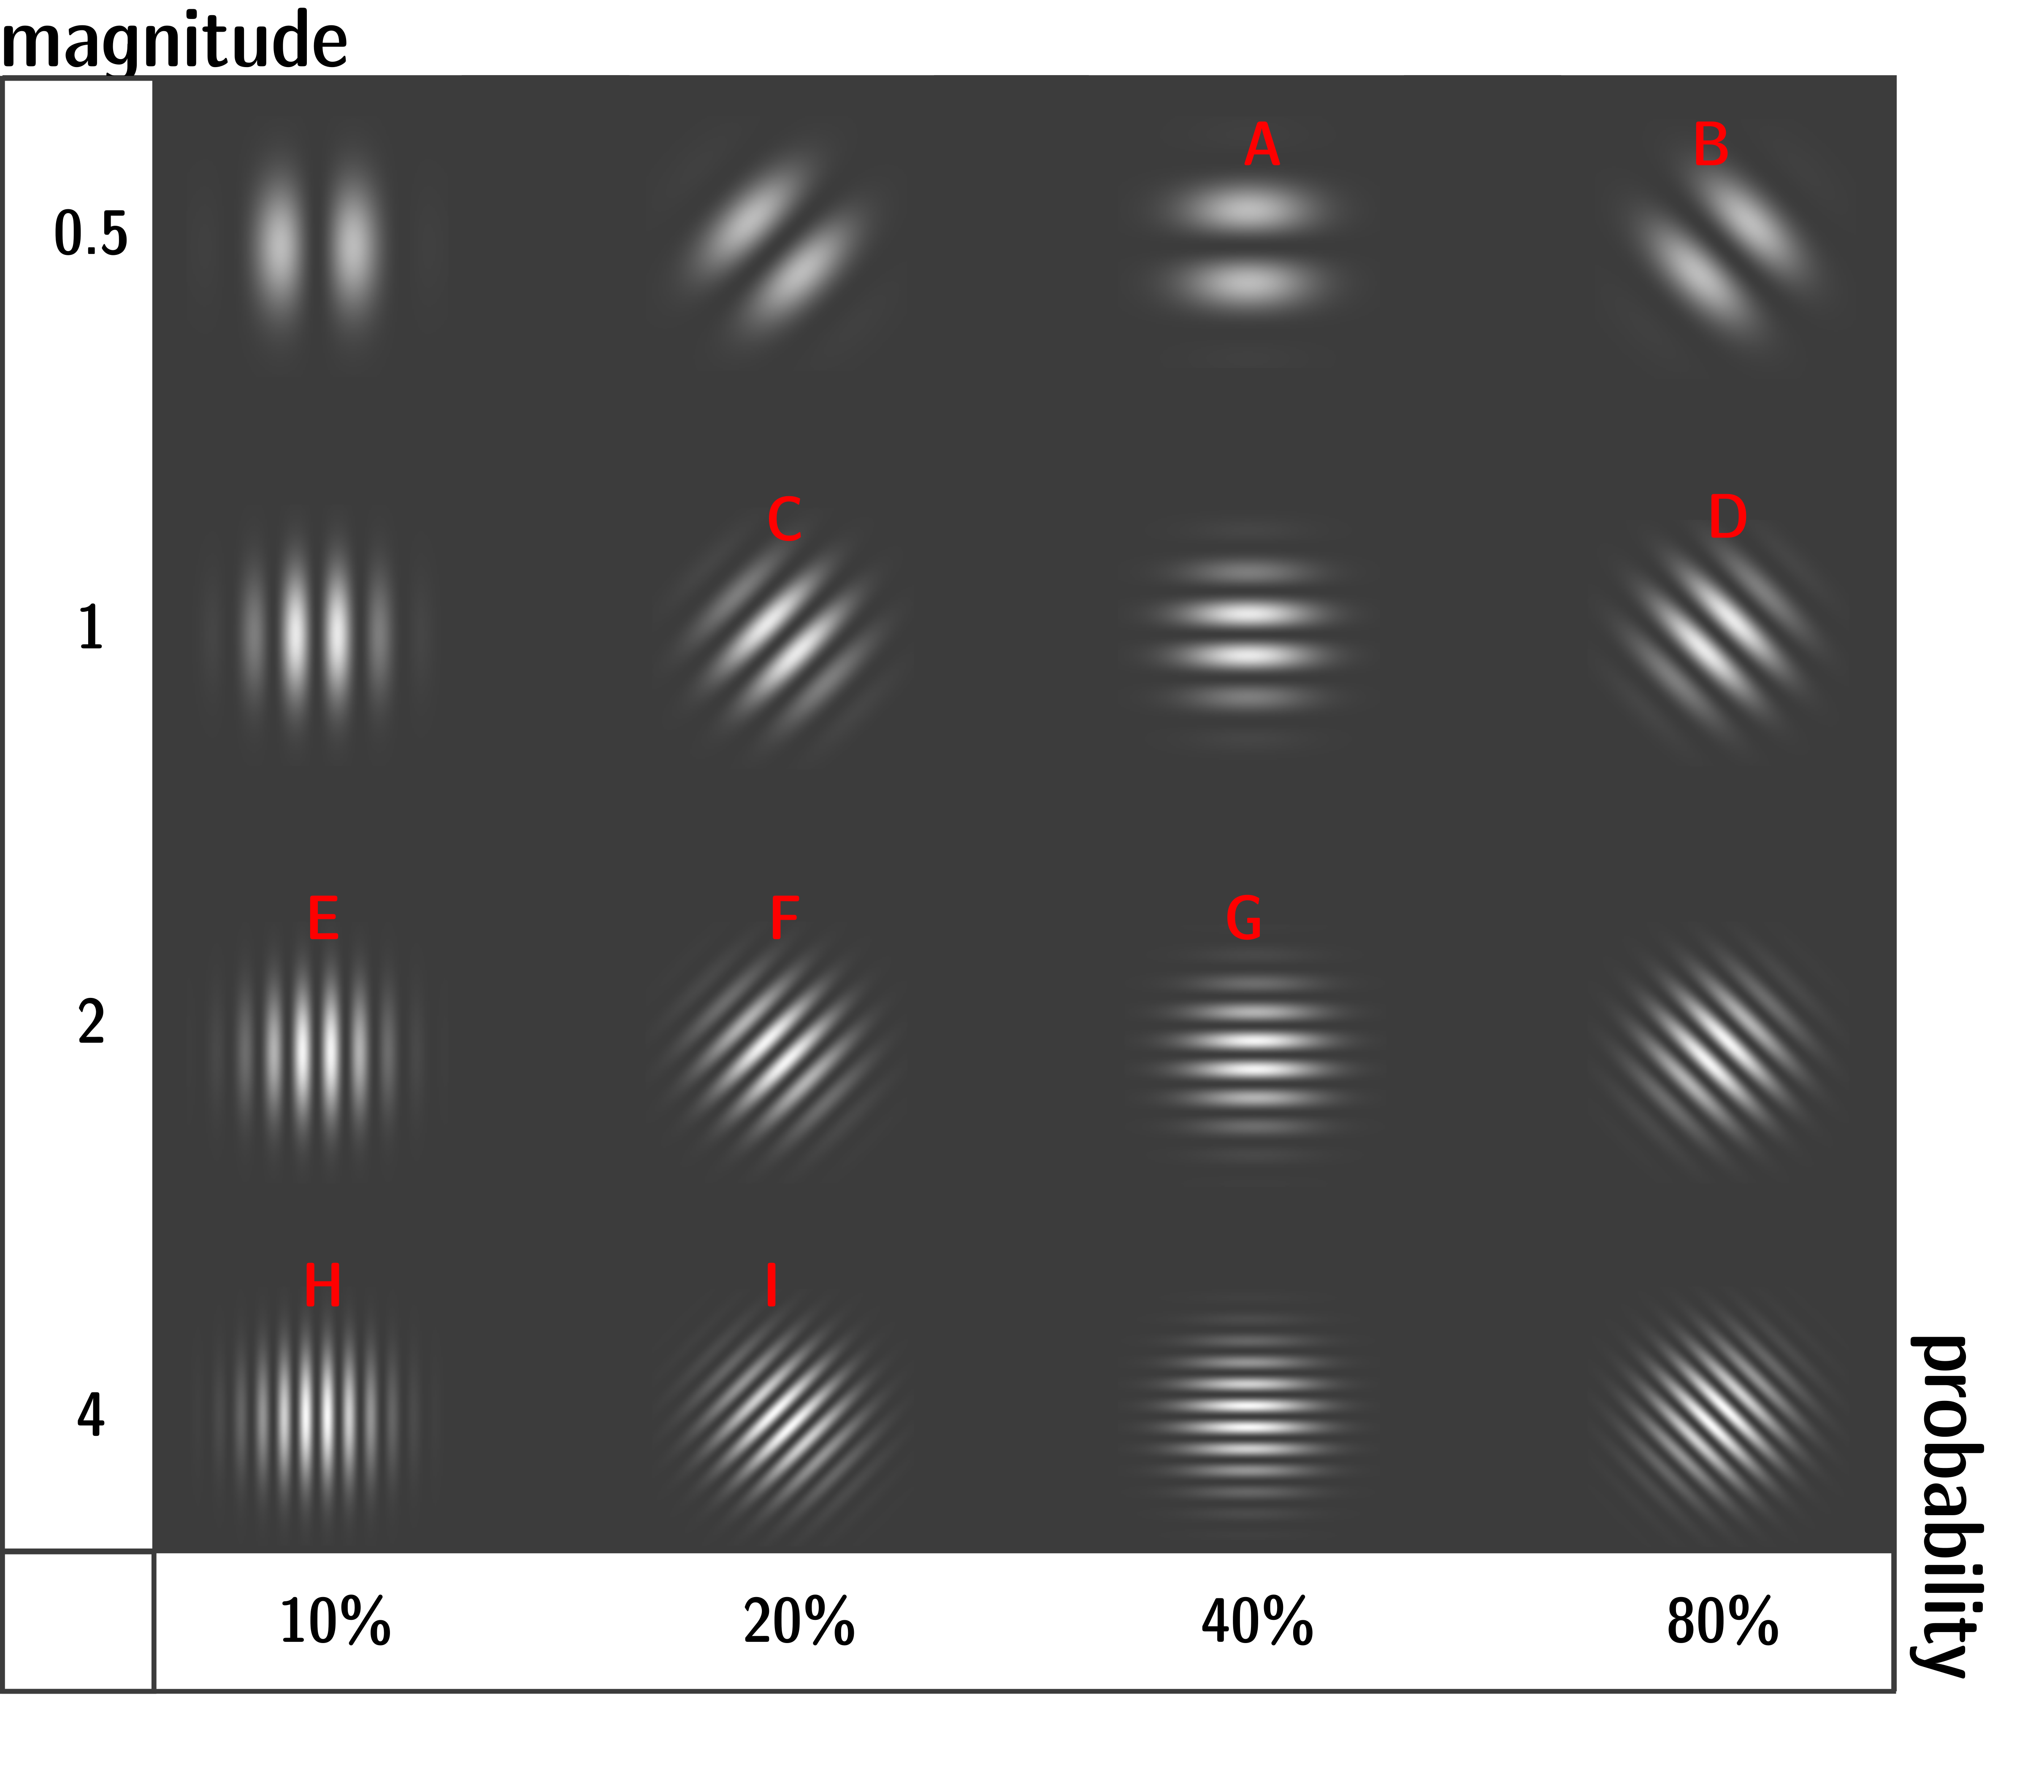
\includegraphics[width=0.5\textwidth]{memento/memento-stimuli.png}
	\caption[Stimulus overview]{Stimulus overview: Gabor patches varied in the number of stripes and their angle, encoding magnitude and probability, respectively. While all presented stimuli were learned in the tutorial, red letters indicate the selection of nine stimulus types used for the left option in the actual experiment. Trials without this annotation were only used intermittent as the right stimulus option to balance the overall expected value between the left and right stimulus option over the course of the experiment.}
	\label{fig:memento_stim}
\end{figure}

\begin{figure}
	\begin{subfigure}{.54\textwidth}
	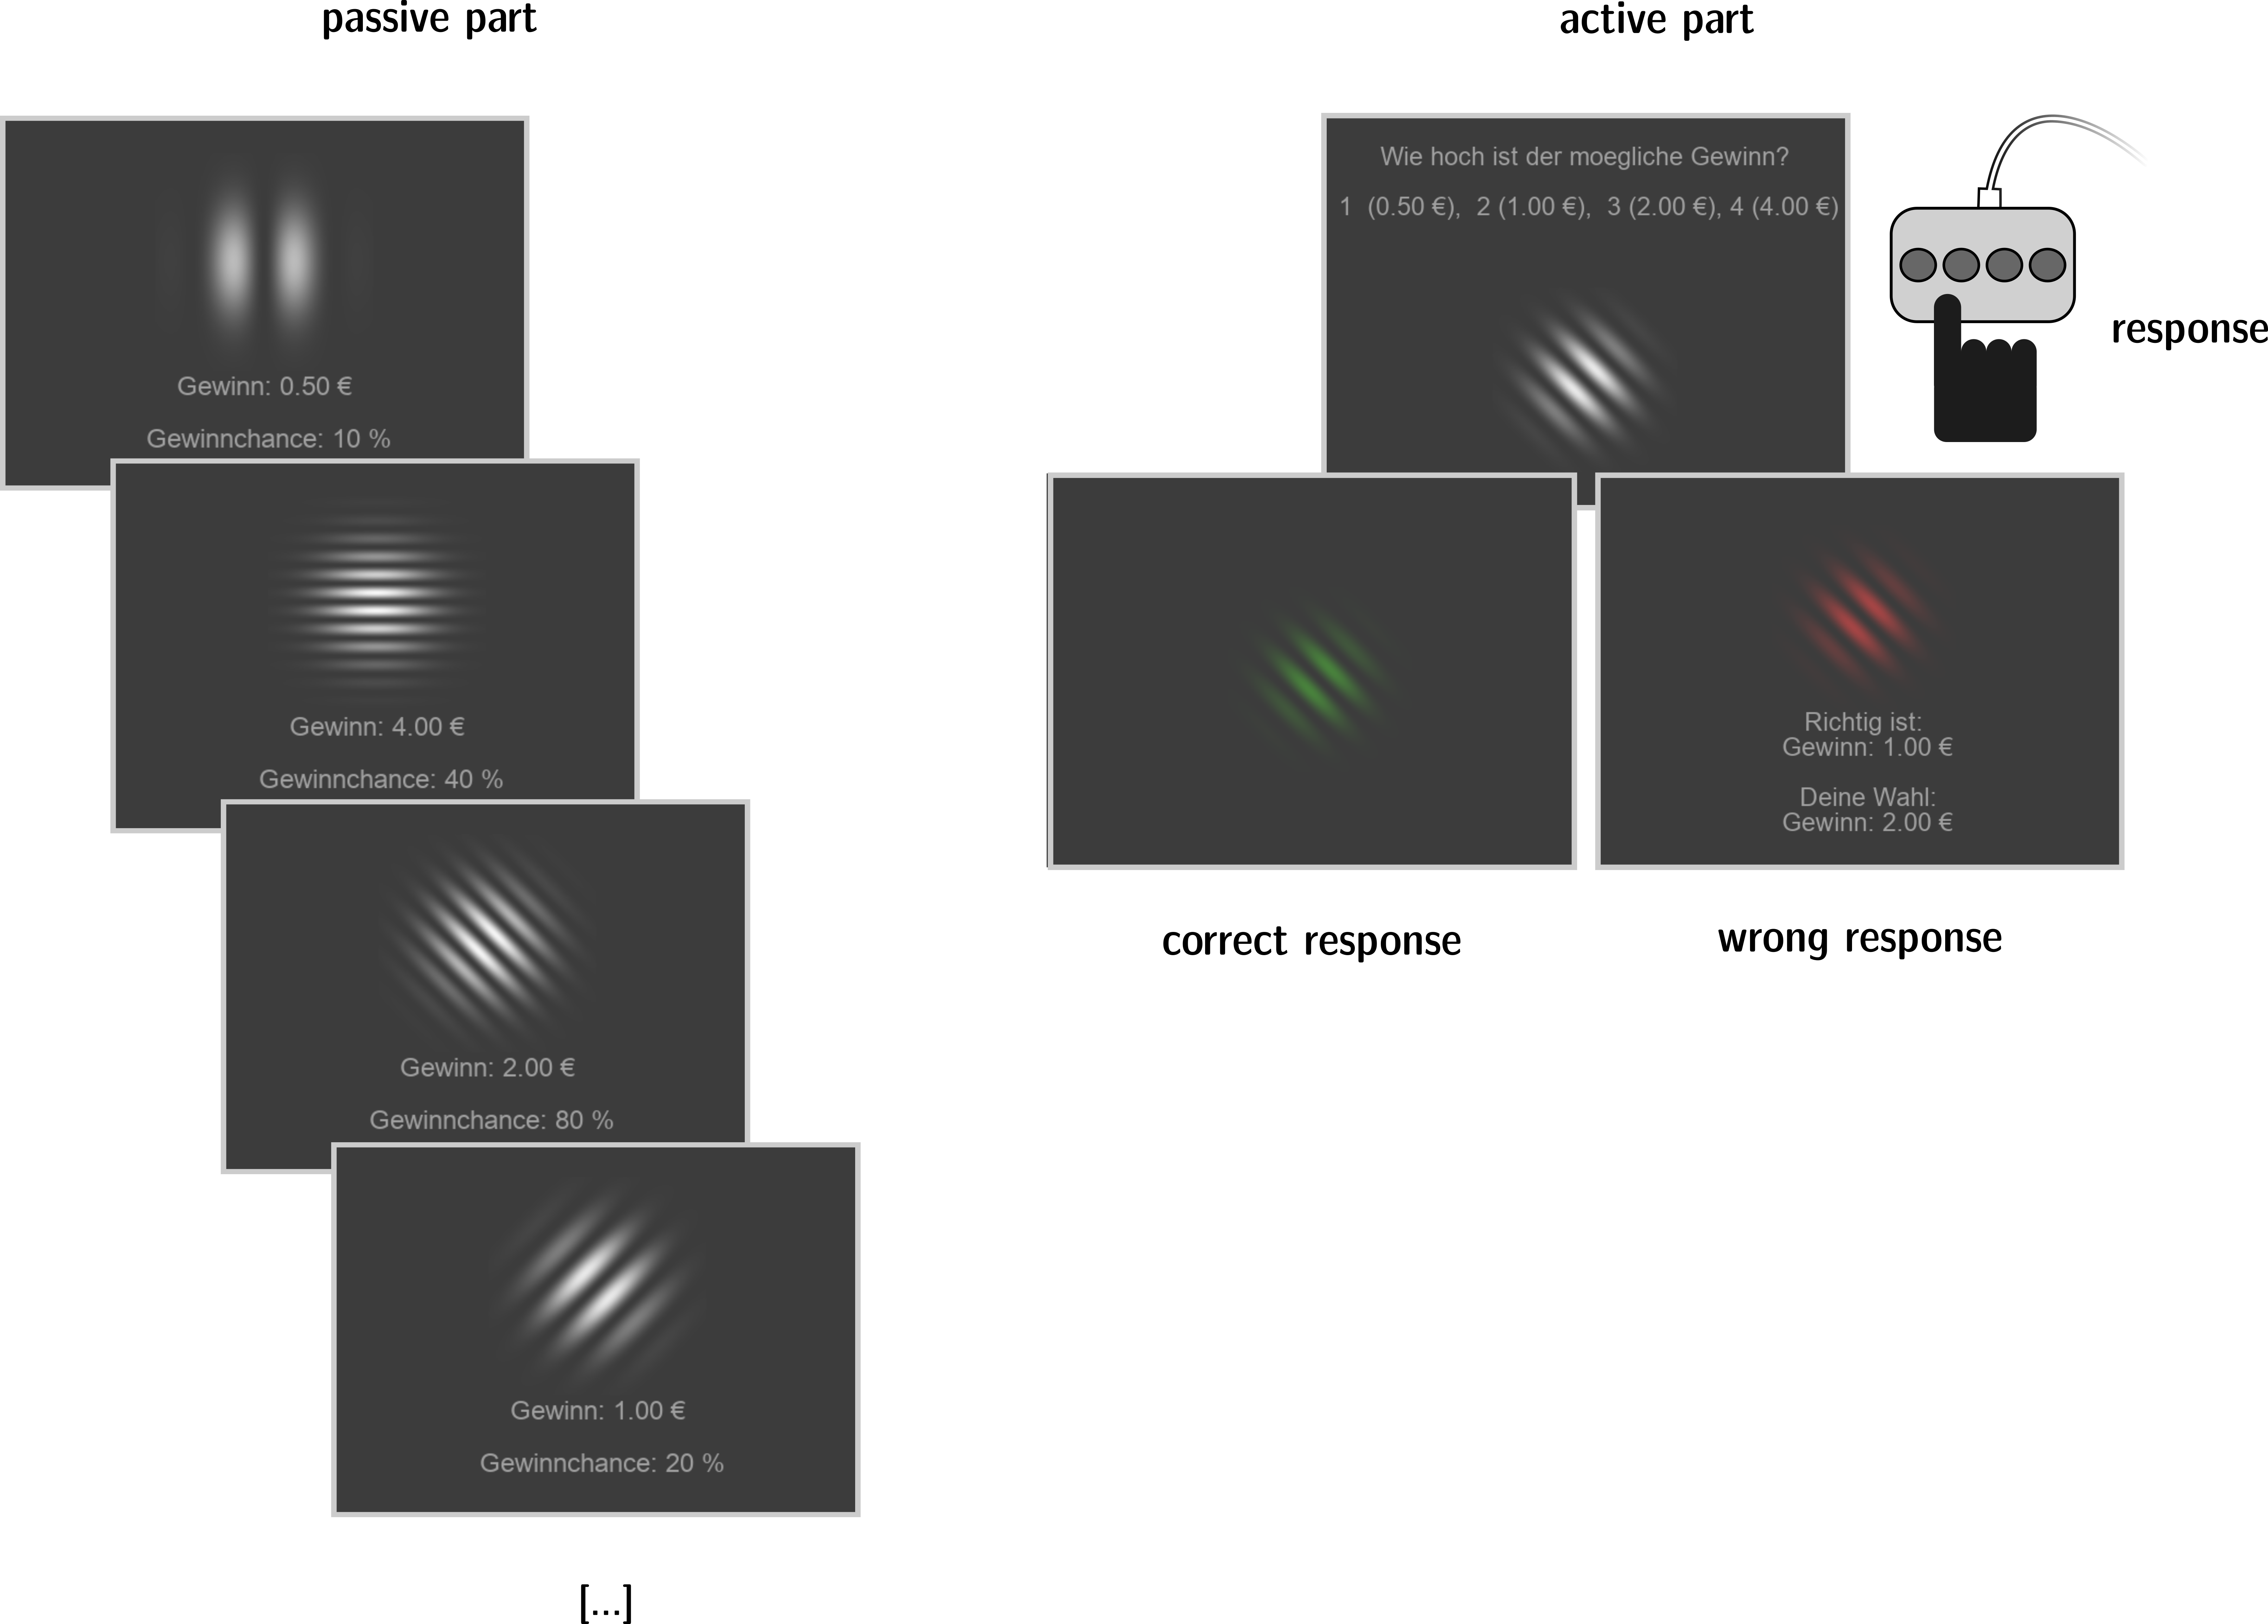
\includegraphics[width=\textwidth]{memento/memento_tutorial.png}
	\caption{Schematic overview of the tutorial.}
	\label{fig:memento_tutorial}
	\end{subfigure}
	\begin{subfigure}{.45\textwidth}
	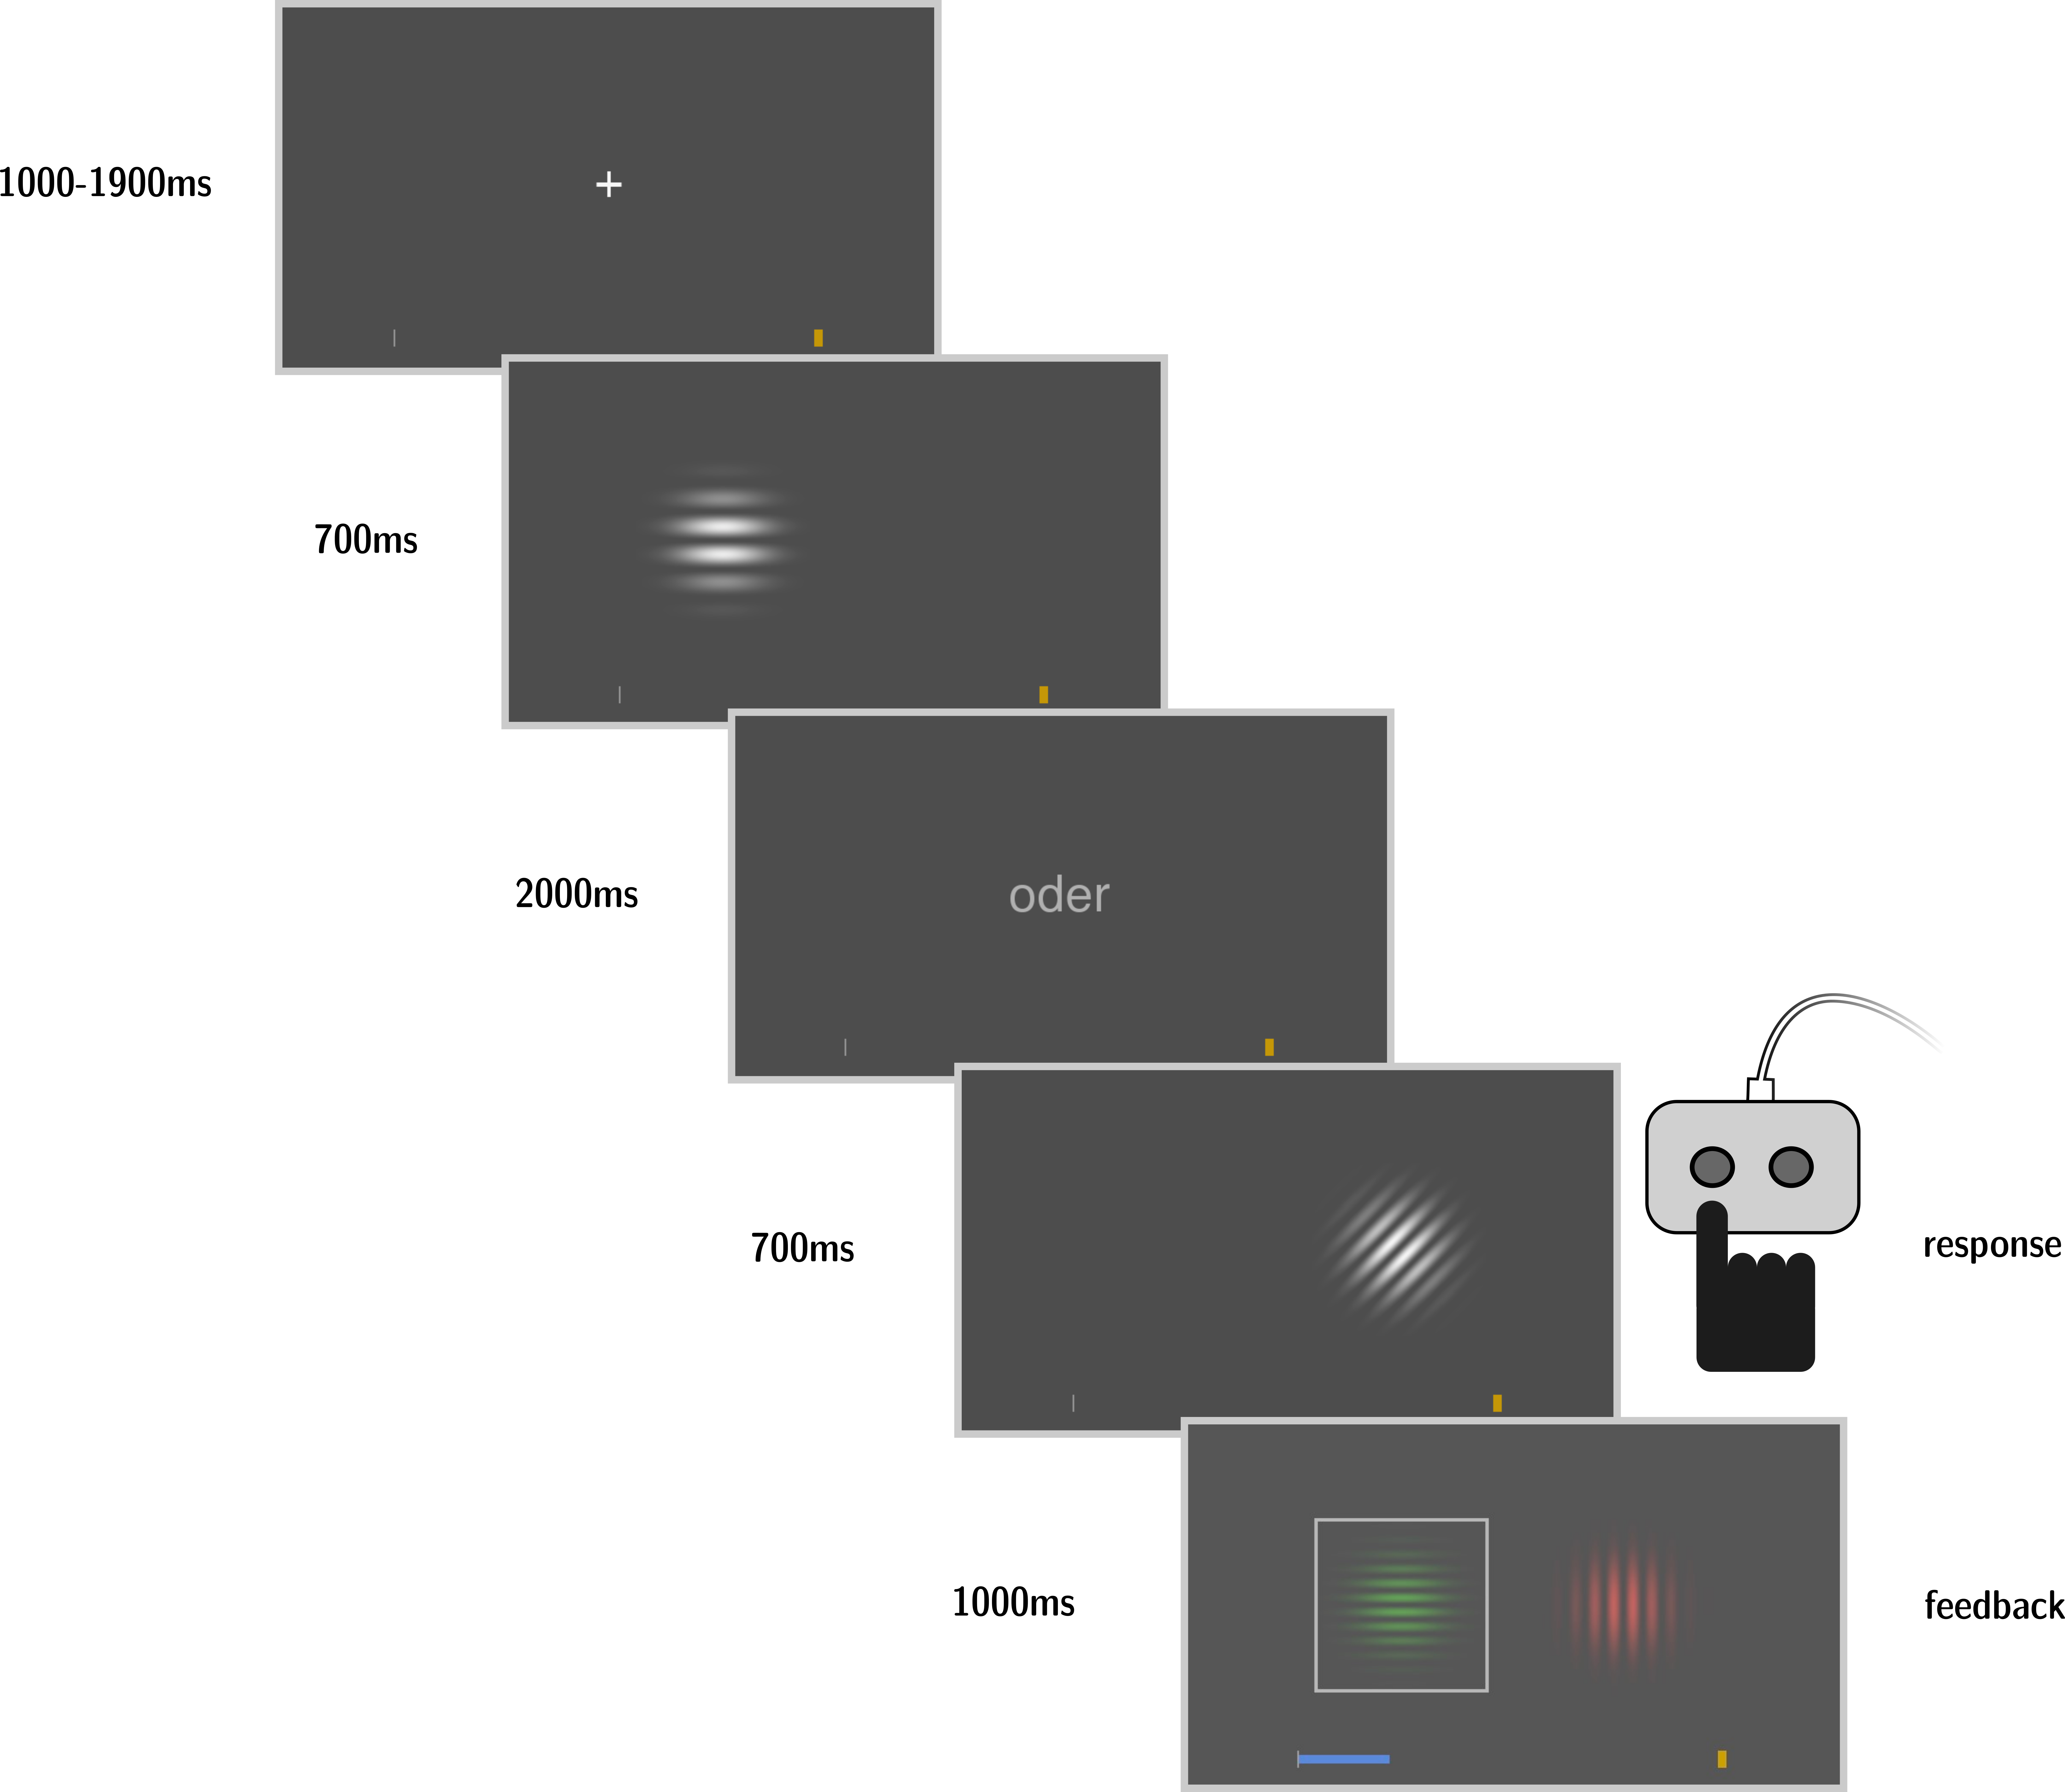
\includegraphics[width=\textwidth]{memento/memento_experiment.png}
	\caption{Schematic overview of a single trial.}
	\label{fig:memento_trial}
\end{subfigure}
	\caption[Memento: Tutorial and trial overview]{Schematic overview of the tutorial (\ref{fig:memento_tutorial}) and a single trial in the experiment (\ref{fig:memento_trial}).
	The tutorial was split in an active and a passive part.
	In the passive part, participants were presented with a stimulus and how its properties translated to reward magnitude and probability. All possible magnitude and probability combinations were presented twice, and participants controlled the pace. The active part then tested participants' knowledge by presenting a stimulus without the annotation. Based on a text prompt, participants had to report its associated magnitude or probability via button press. They received feedback with a green colored stimulus for a correct response, or, for an incorrect response, a red colored stimulus together with a report of their response versus the true response.
	}
\label{fig:memento}
\end{figure}


\subsection{MEG acquisition}

Following a metal test, MEG data were acquired on an Elekta Neuromag TRIUX System with internal helium recycler and 306 sensors (204 planar gradiometers and 102 magnetometers) in a magnetically shielded room.
Participants were instructed to take a comfortable seating position and sit as still as possible.
The experiment was presented on a screen in a distance of one meter from the sitting participants via a projector with a refresh rate of 60 Hz located outside the MEG recording chamber.
Additional sensors captured confounding biological signals:
Lateral and vertical eye movements and blinks were captured using electrooculography surface electrodes on the tori supra- and infraorbitalis and next to the external canthi.
Heartbeat artifacts were recorded with an electrocardiogram.
Head position indicator coils captured the participants head movements.
Behavioral responses were registered using an MEG compatible keyboard.
The neural data was recorded at a sampling rate of 1000Hz and active internal shielding (IAS).


\subsection{Preprocessing}

Prior to preprocessing, raw data were restructured to \gls{BIDS} format (v1.4.0) using mne-bids \citep{Appelhoff2019}.
Simultaneously, behavioral log files were transformed from proprietary .mat into the TSV format.

As the first step of preprocessing, the spatiotemporal extension of the \gls{SSS} method \citep{taulu2005presentation}, \textit{\gls{tSSS}} \citep{taulu2006spatiotemporal}, was applied, as is common for recordings on Neuromag MEG systems with active internal shielding.
\gls{SSS} and \gls{tSSS} remove strong interference from external noise sources and sources within the body itself from the MEG signal.
The methods can be applied on whole-scalp multichannel data when the precise sensor calibrations are known, and were initially developed as the proprietary MaxFilter\textsuperscript{TM} algorithm by Elekta Neuromag.
To this end, Neuromag systems provide a cross-talk compensation and fine calibration file which reduces interference between their co-located magnetometer and paired gradiometer sensor units and encodes site-specific information about sensor orientation and calibration, respectively.
Based on the Maxwell equations \citep{taulu2006spatiotemporal}, \gls{SSS} decomposes \gls{meg} signals ($\phi$) into elementary magnetic fields from sources within the sensor helmet (the \textit{internal} subspace) and into an orthogonal set for fields arising from sources outside (the \textit{external} subspace).

\begin{equation}
	\begin{aligned}
	  \phi = \sum_{l=1}^{\inf}\sum_{m=-l}^{l} \alpha_{lm} a_{lm} + \sum_{l=1}^{L_{out}}\sum_{m=-l}^{1}\beta_{lm}b_{lm}
	\end{aligned}
\label{eq:sss}
\end{equation}

Based on this, it transforms the $N=306$-dimensional signal vector into a lower dimensional subspace that spans all measurable signals, the ``SSS basis'' $S$. Its subspaces $S_in$ and $S_out$ contain the biomagnetic signal and arbitrary external interference, respectively.

\begin{equation}
	\begin{aligned}
		    \phi &= S_x = [S_{in} S_{out}] \begin{bmatrix}
			x_{in} \\
			x_{out}
		\end{bmatrix}
	\end{aligned}
	\label{eq:sss}
\end{equation}

The SSS basis is $n=(L_{in}+1)^2+(L_{out}+1)^2$-dimensional, with typical model orders $L_{in}=8$ and $L_{out}=3$, resulting in $n=95$ (80 internal, 15 external) dimensions.
With $n \ll N$, $\phi$ can be uniquely decomposed into internal and external components

\begin{equation}
	\begin{aligned}
			\phi &= S_x = [S_{in} S_{out}] \begin{bmatrix}
			x_{in} \\
			x_{out}
		\end{bmatrix} = \phi_{in} + \phi_{out}
	\end{aligned}
	\label{eq:sss}
\end{equation}

As the internal and external subspaces are provably linearly independent, brain signals are then reconstructed by retaining only sources inside the helmet, thus excluding external inferences.


\begin{equation}
	\begin{aligned}
    \hat{x} =
\begin{bmatrix}
	\hat{x}_{in} \\
	\hat{x}_{out}
\end{bmatrix}
= S^{\dagger}\phi \\
\hat{\phi}_{in} = S_{in}\hat{x}_{in}\\
	\end{aligned}
	\label{eq:sss}
\end{equation}


According to \citet{taulu2006spatiotemporal}, \gls{SSS} can separate brain signals from sources >0.5m away, suppressing external interference by a factor >100.
The spatiotemporal extension \gls{tSSS} can further detect inferences from closer sources such as stimulators or pacemakers.
These are estimated based on the fact that their strength typically exceeds that of sensor noise and they thus, unlike brain signal, leak into both the internal and external part of the \gls{SSS} reconstruction.
After detecting components with a high temporal correlation between the external and internal subspaces, \gls{tSSS} removes close-by artifacts by projecting the components common to the internal and external subspace out of the internal subspace.
In the absence of nearby artifacts, \gls{tSSS} reduces to \gls{SSS} \citep{taulu2009removal}.
\gls{tSSS} was implemented using mne-python's open source implementation \texttt{maxwell\_filter()} with a chunk duration of 10 seconds and a correlation threshold of at least $0.98$.
Prior to \gls{tSSS}, bad channels were detected and annotated automatically in order to prevent bad channel noise from spreading.
To compensate for head movements, measurements from the head position indicator coils were used to estimate subject motion, and motion correction was then performed as part of the \gls{tSSS} procedure: As the signal representation in the \gls{SSS} basis is device independent, internal data can simply be transformed to a sensor array corresponding to the average head position.
After \gls{tSSS}, gradiometers and magnetometers contain highly similar information and have an altered inter-channel correlation structure because they were reconstructed from a common 80-dimensional subspace \citep{jas2018reproducible}.
Formerly bad channels have also been effectively repaired by the procedure.
After \gls{tSSS}, some spectral artifacts remained in the data, among them power line noise at 50Hz and a spectral peak at 60Hz, likely originating from the presentation screen's refresh rate.
ZAPline filtering \citep{de2020zapline} was performed to remove them using \texttt{meegkit} \citep{barascud2022}.
Figures \ref{fig:prezap} and \ref{fig:postzap} show power spectral density plots of the signal pre and post (effective window size: 2.048 s) applying ZAPline filters.


\begin{figure}
	\begin{subfigure}{.49\textwidth}
		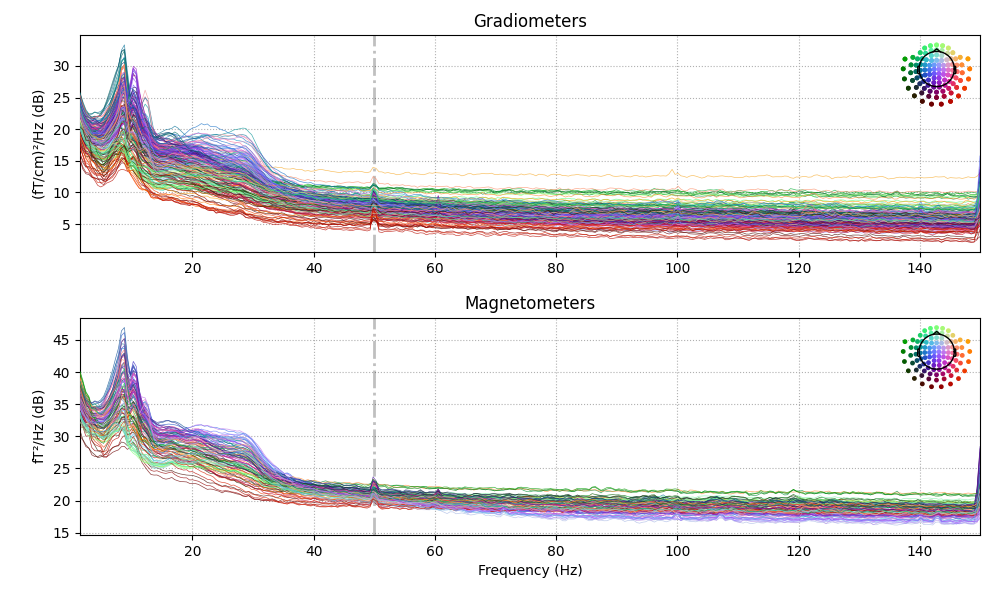
\includegraphics[width=\textwidth]{memento/psd_pre_zapline.png}
		\caption{Power spectral density before ZAPline filtering}
		\label{fig:prezap}
	\end{subfigure}
	\begin{subfigure}{.49\textwidth}
		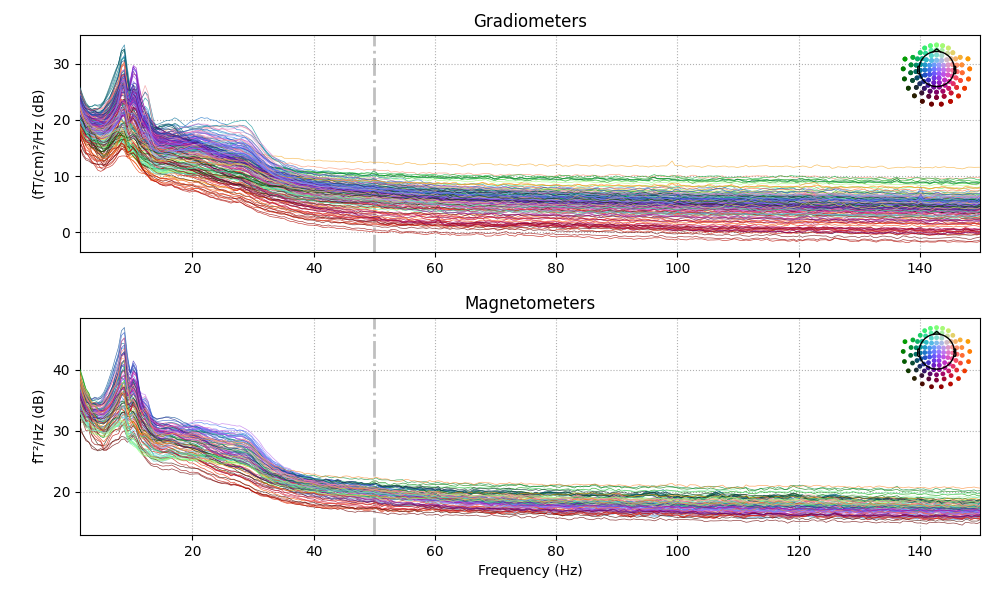
\includegraphics[width=\textwidth]{memento/psd_post_zapline.png}
		\caption{Power spectral density after ZAPline filtering}
		\label{fig:postzap}
	\end{subfigure}
	\caption[Power spectral density before and after ZAPLine filtering]{Power spectral density of all MEG channels
		from a single subject before (\ref{fig:prezap}) and after (\ref{fig:postzap}) ZAPLine filtering.
		Two spikes at 50Hz (power-line frequency) and 60Hz (likely an artifact of the stimulus presentation) are markedly reduced afterwards.
	}
	\label{fig:zapline_psd}
\end{figure}

Next, data were first low-pass filtered with a 100Hz lowpass FIR filter to constrain it into a frequency range of interest.
The filter properties are reported in \ref{fig:preproc} and a visualization is in \ref{fig:filter}.
As eye movements, eye blinks, heart beats, and facial muscle contractions survive \gls{tSSS}, \gls{ica} was used to detect and remove these artifacts.
% The slow drifts are problematic because they reduce the independence of the assumed-to-be-independent sources (e.g., during a slow upward drift, the neural, heartbeat, blink, and other muscular sources will all tend to have higher values), making it harder for the algorithm to find an accurate solution. A high-pass filter with 1 Hz cutoff frequency is recommended. However, because filtering is a linear operation, the ICA solution found from the filtered signal can be applied to the unfiltered signal https://ieeexplore.ieee.org/document/7319296/
As ICA is sensitive to low-frequency drifts \citep{winkler2015ICA}, the data were first processed with a temporary one-pass, zero-phase, non-causal highpass filter (firwin method, Hamming window with 0.0194 passband ripple and 53 dB stopband attenuation, a lower passband edge of 1.00, lower transition bandwidth of 1.00 Hz (-6 dB cutoff frequency: 0.50 Hz), and a filter length of 3301 samples (3.301 s)).
As ICA can further be sensitive to bad segments in the recording, data were temporarily epoched into 5 second splits from the onset of the fixation cross.
\texttt{autoreject} was then used on the first 200 of these epochs to estimate the noise level and compute rejection thresholds.
Afterwards, FastICA \citep{hyvarinen1999fast} was used to decompose the signal into 45 independent components.
For most subjects, components corresponding to ECG activity were identified using cross-trial phase statistics \citep{dammers2008integration} with an automatically computed threshold of 0.16 for the Kuiper statistic, and EOG related components were found using Pearson correlation.
For one subject, however, the ECG channel was flat, and components were manually selected.
Afterwards, the ICA solution was applied to the continuous recording and detected ECG and EOG components were zeroed out.

As a final step, the continous recording was chunked into Epochs of varying length depending on analysis, and \texttt{autoreject} was used to detect and repair or drop bad epochs.
Figure \ref{fig:preproc} summarizes the preprocessing steps.
Figure \ref{fig:cleanepoch} shows an average of cleaned 5 second epochs for a single subject.



\begin{figure}
	\begin{subfigure}{0.4\textwidth}
		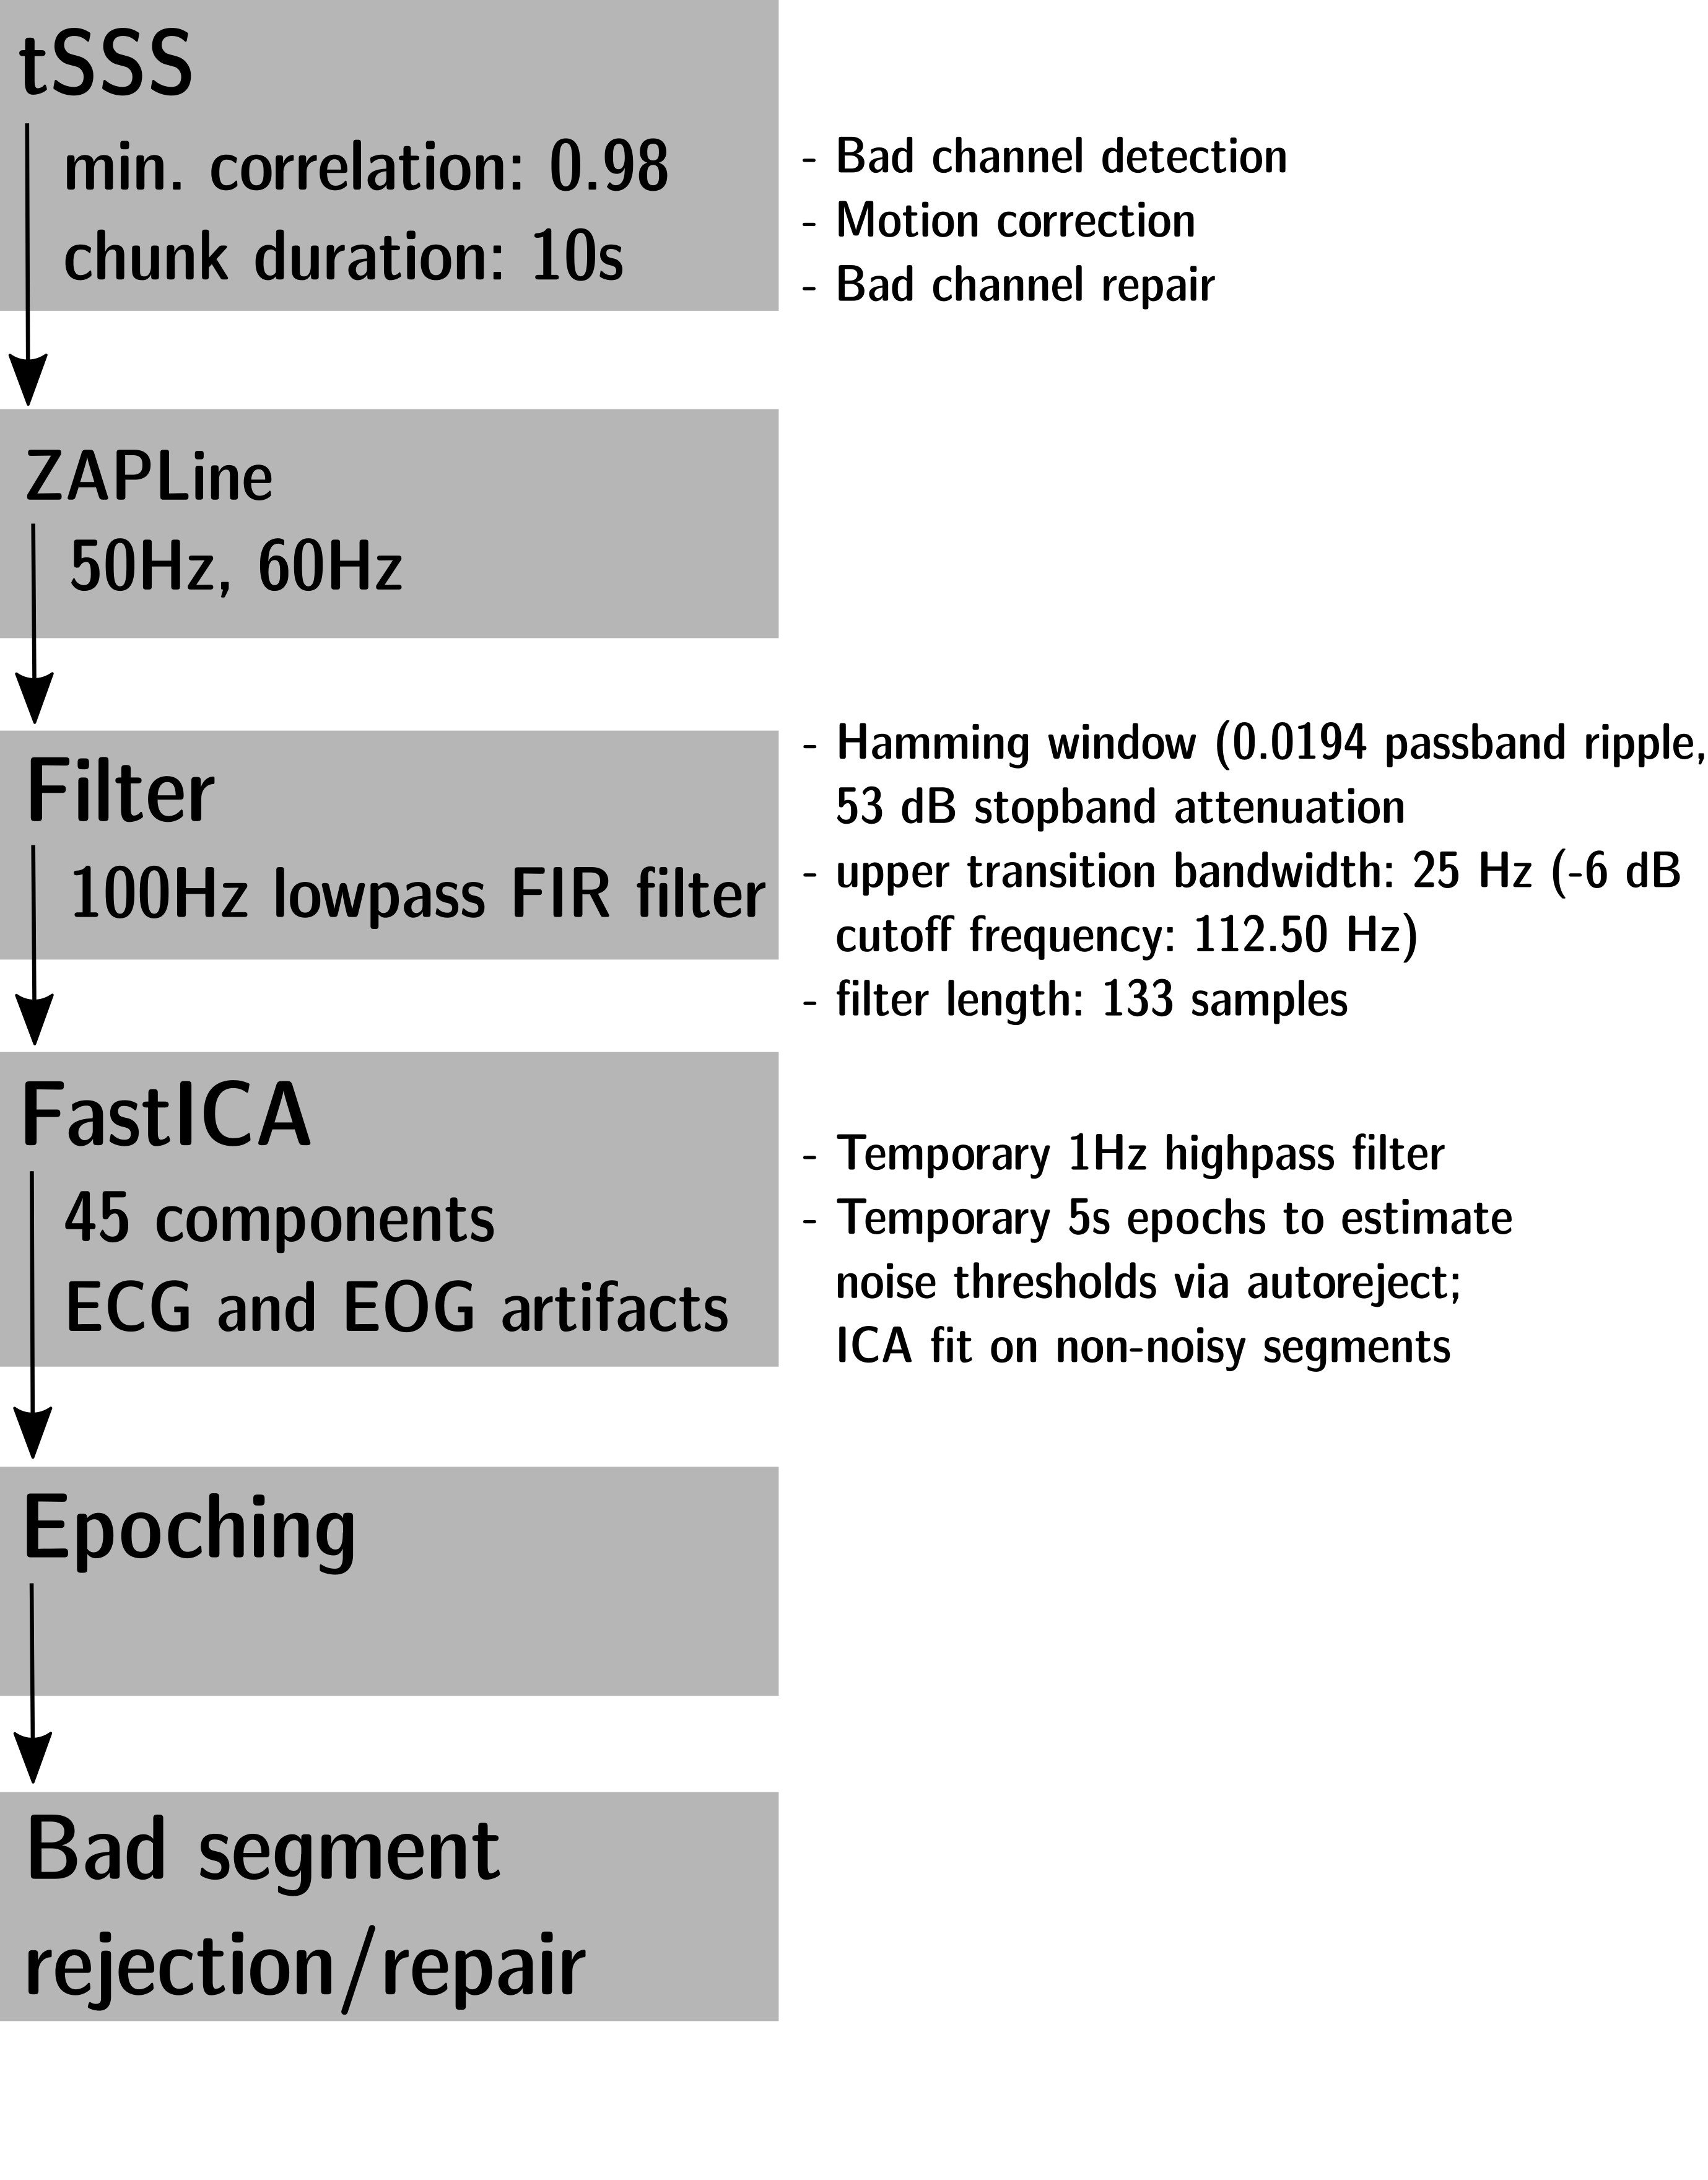
\includegraphics[width=\textwidth]{memento/preprocessing_overview.png}
		\caption[Preprocessing overview]{Preprocessing Overview}
		\label{fig:preproc}
	\end{subfigure}
	\begin{subfigure}{0.4\textwidth}
		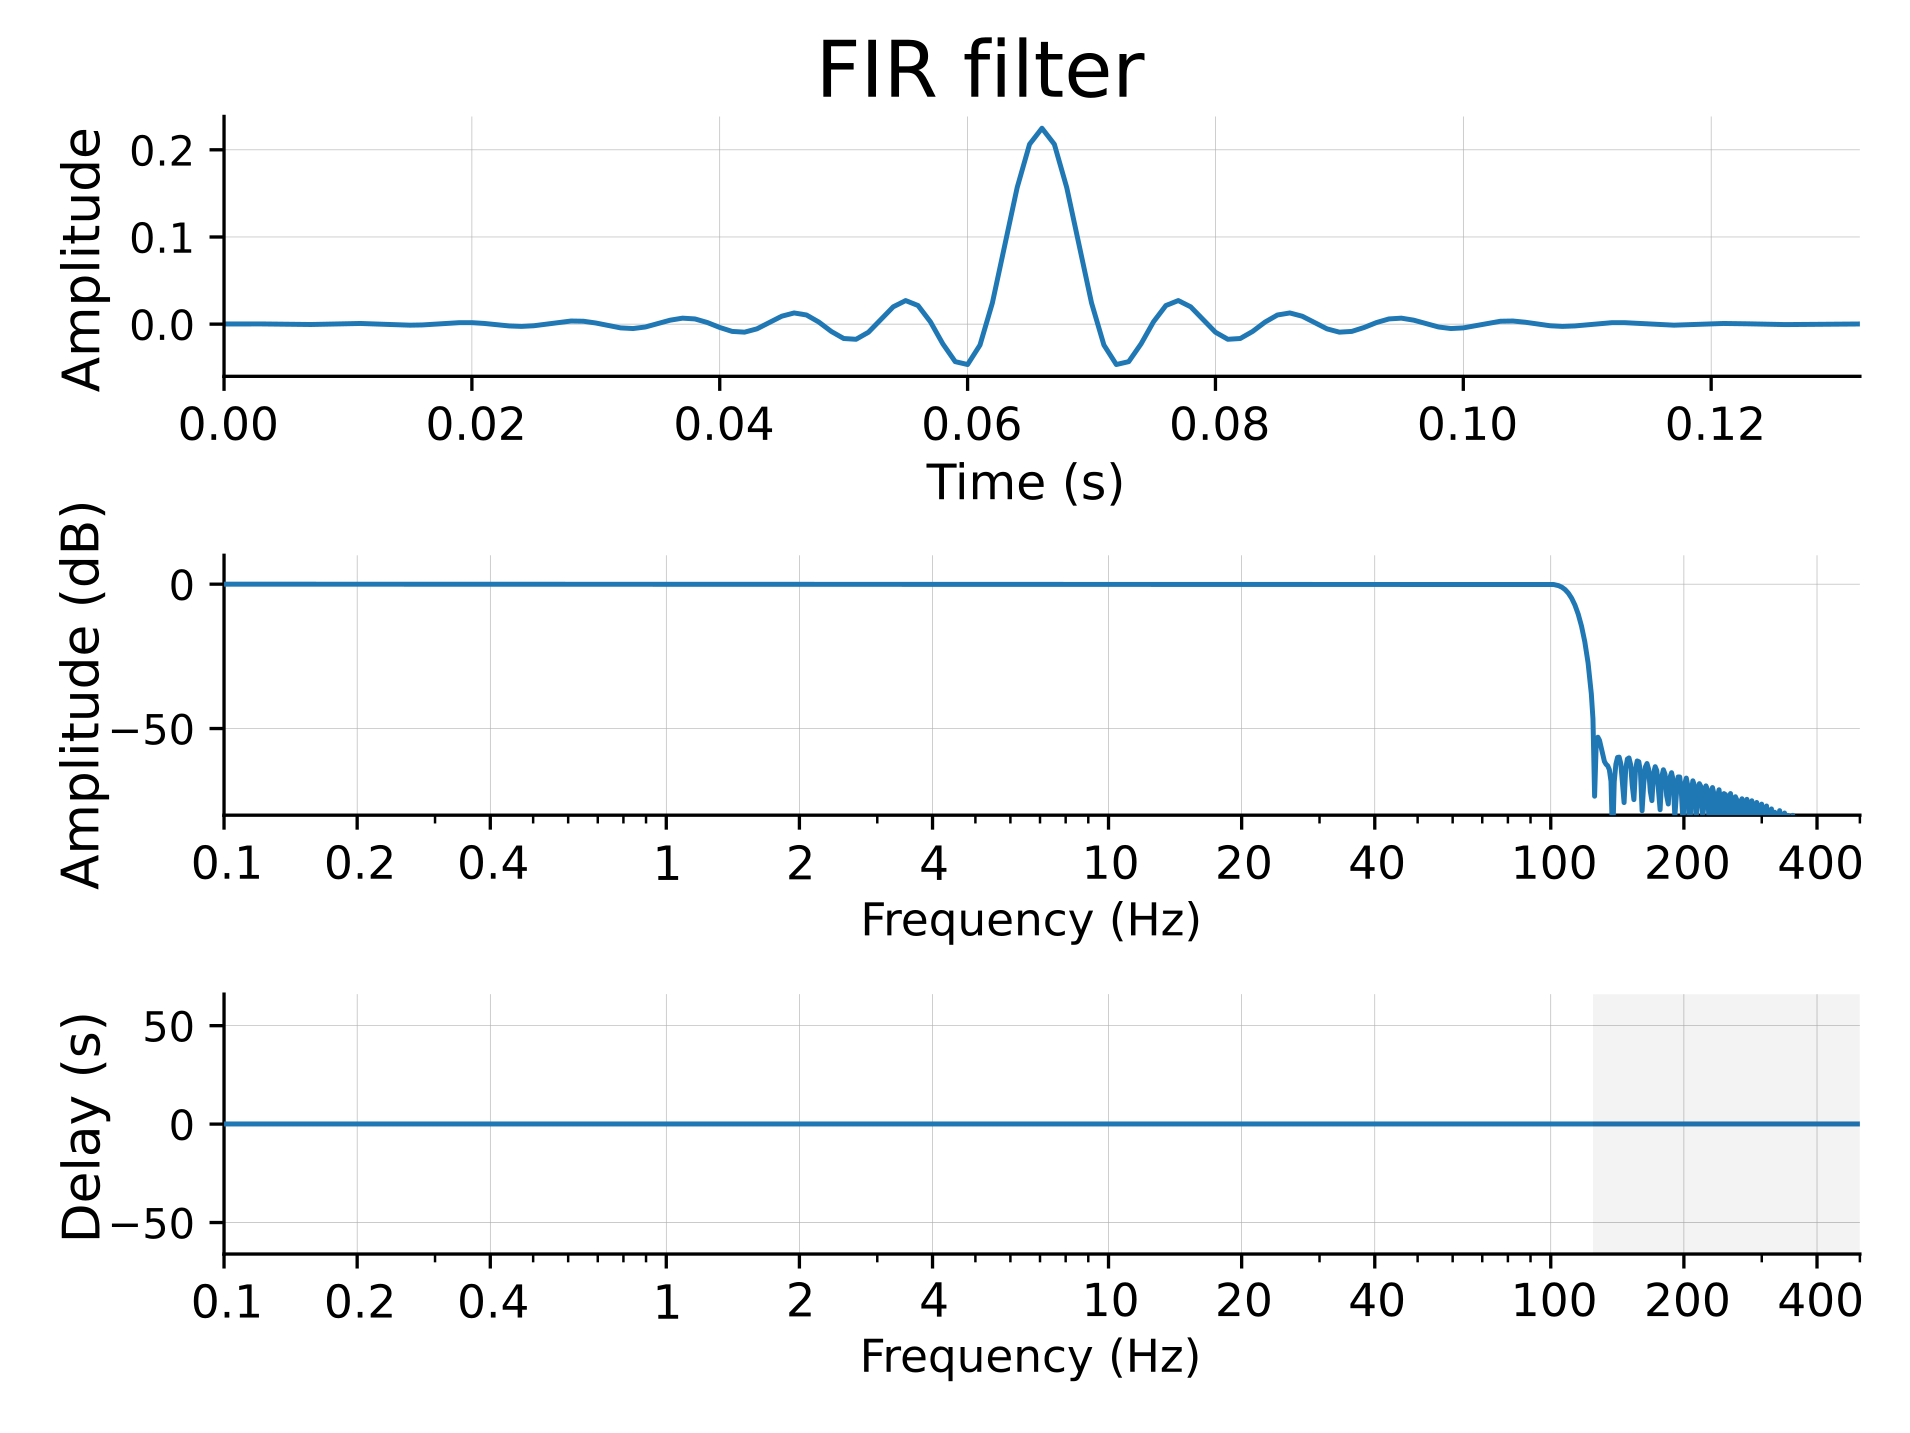
\includegraphics[width=\textwidth]{memento/filter_properties_100hz.png}
		\caption[Lowpass filter properties]{Lowpass filter properties}
		\label{fig:filter}
	\end{subfigure}
	\caption[Preprocessing]{Preprocessing thingies}
\end{figure}

\begin{figure}
	\centering
	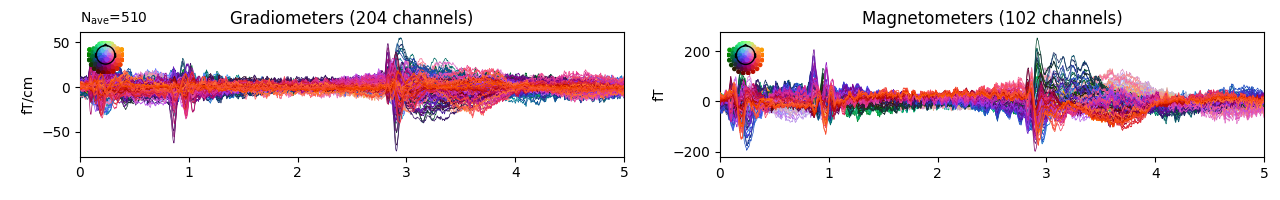
\includegraphics[width=0.5\textwidth]{memento/average_epoch_cleaned.png}
	\caption[Average neural signal over the trial course]{Neural recordings from a single exemplary subject.
		Shown is the average of cleaned epochs with a length of 5 seconds from left stimulus onset, corresponding to a trial from first visual stimulation until
		1600ms after the offset of the second stimulus.}
	\label{fig:cleanepoch}
\end{figure}

All preprocessing steps and the subsequent analysis were implemented using mne python (CITE) or custom Python functions. All preprocessing and analysis scripts are openly available on GitHub and as the python package \texttt{pymento\_meg} (CITE).


\pagebreak

\section{Shared response modeling}

% This needs a general introduction into shared response modeling
The underlying assumption of functional alignment methods is that brain activity can be modeled in an n-dimensional space, where n is the number of measurements (e.g., voxels in \gls{fMRI}, sensors in \gls{meg}, or electrodes in \gls{eeg} acquisitions).
When subjects experience the same events, their brain activity may differ anatomically, but should correspond to similar cognitive processes.
To functionally align the brain activity of multiple participants, we align the vector representations of their brain signals.
Afterwards, we need to assign meaning to the axes of the shared space.

During \gls{tSSS}, the neural signal is decomposed from the 306 dimensional sensor space into an 80-dimensional subspace, the \gls{SSS} basis.
This confirms that the signal of interest can be expressed in fewer than 306 dimensions.
We therefore sought to find out whether we can find meaningful low-dimensional structure in the high-dimensional dataset via \gls{SRM} \citep{NIPS2015_b3967a0e}.

In \gls{SRM}, the objective is to model each subject $i$'s response to temporally synchronized stimuli as a subject-specific base $W_i$ and a shared component over all subject's responses $S$.
In an \gls{meg} acquisition, each subject $i$ has a data matrix of dimensions sensors $\times$ time-points.


\begin{equation}
	\begin{aligned}
    X_i \in \mathbb{R}^{s \times d}
	\end{aligned}
	\label{eq:sss}
\end{equation}

\gls{SRM} estimates a $k$-dimensional shared space $S$, and orthogonal-column basis vectors of the shared response in subject-space  $\{W_i\}^m_{i=1}$  $\{W_i\}^m_{i=1}$


\begin{equation}
	\begin{aligned}
	    min_{w_i, s}\sum_i{\|X_i - W_iS \|}^2_F \\
	s.t. W^T_iW_i = I_k
	\end{aligned}
	\label{eq:sss}
\end{equation}


\begin{figure}
	\centering
	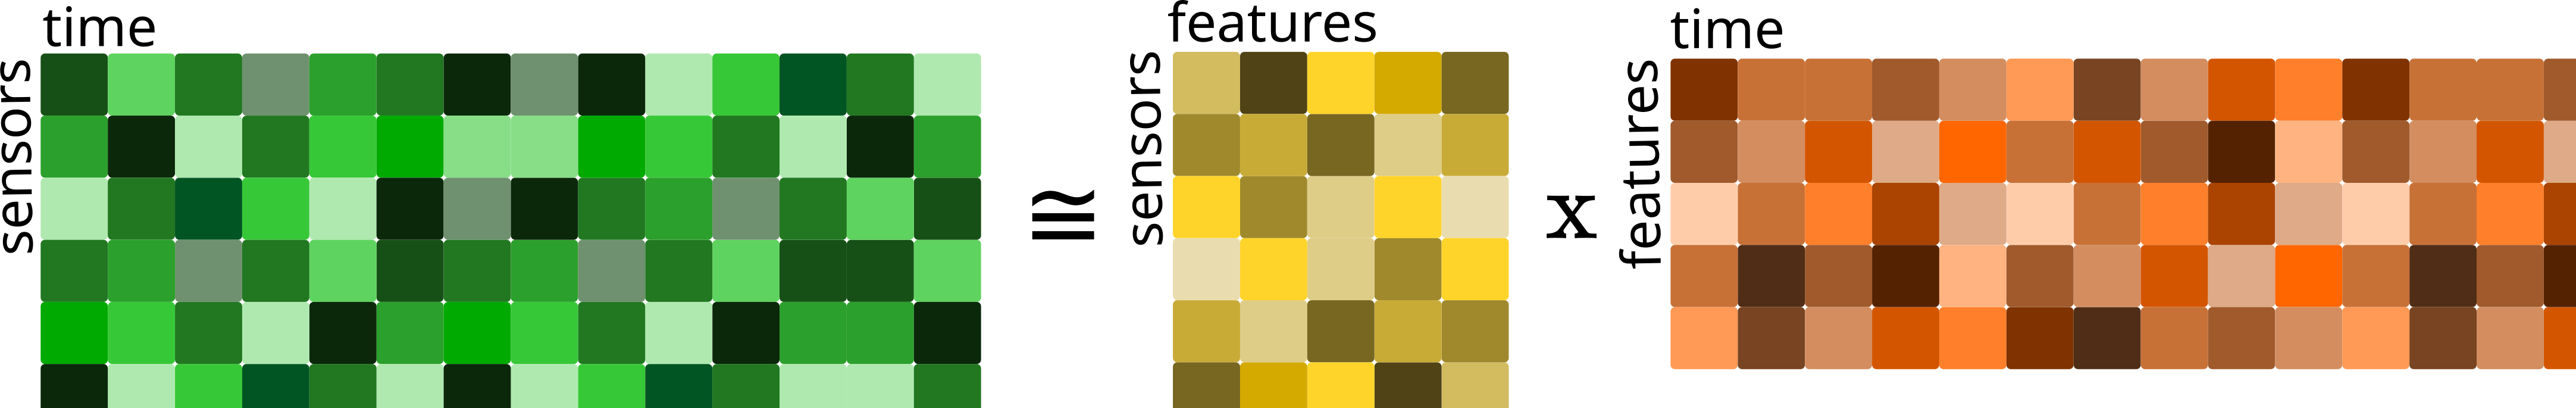
\includegraphics[width=0.9\textwidth]{memento/srm/srm_basics_1.png}
	\caption[SRM overview]{In \gls{SRM} on \gls{meg} data, sensor-by-time matrices are decomposed into a orthogonal subject specific basis matrix (sensor-by-features), a common shared feature matrix (features-by-time), and a subject-specific error}
	\label{fig:srm-basics}
\end{figure}

Given subjects experience the same sequence on stimulus events, \gls{SRM} identifies common activity patterns across subjects, and provides a method to transform the original activity into a shared latent component space.


\begin{figure}
	\centering
	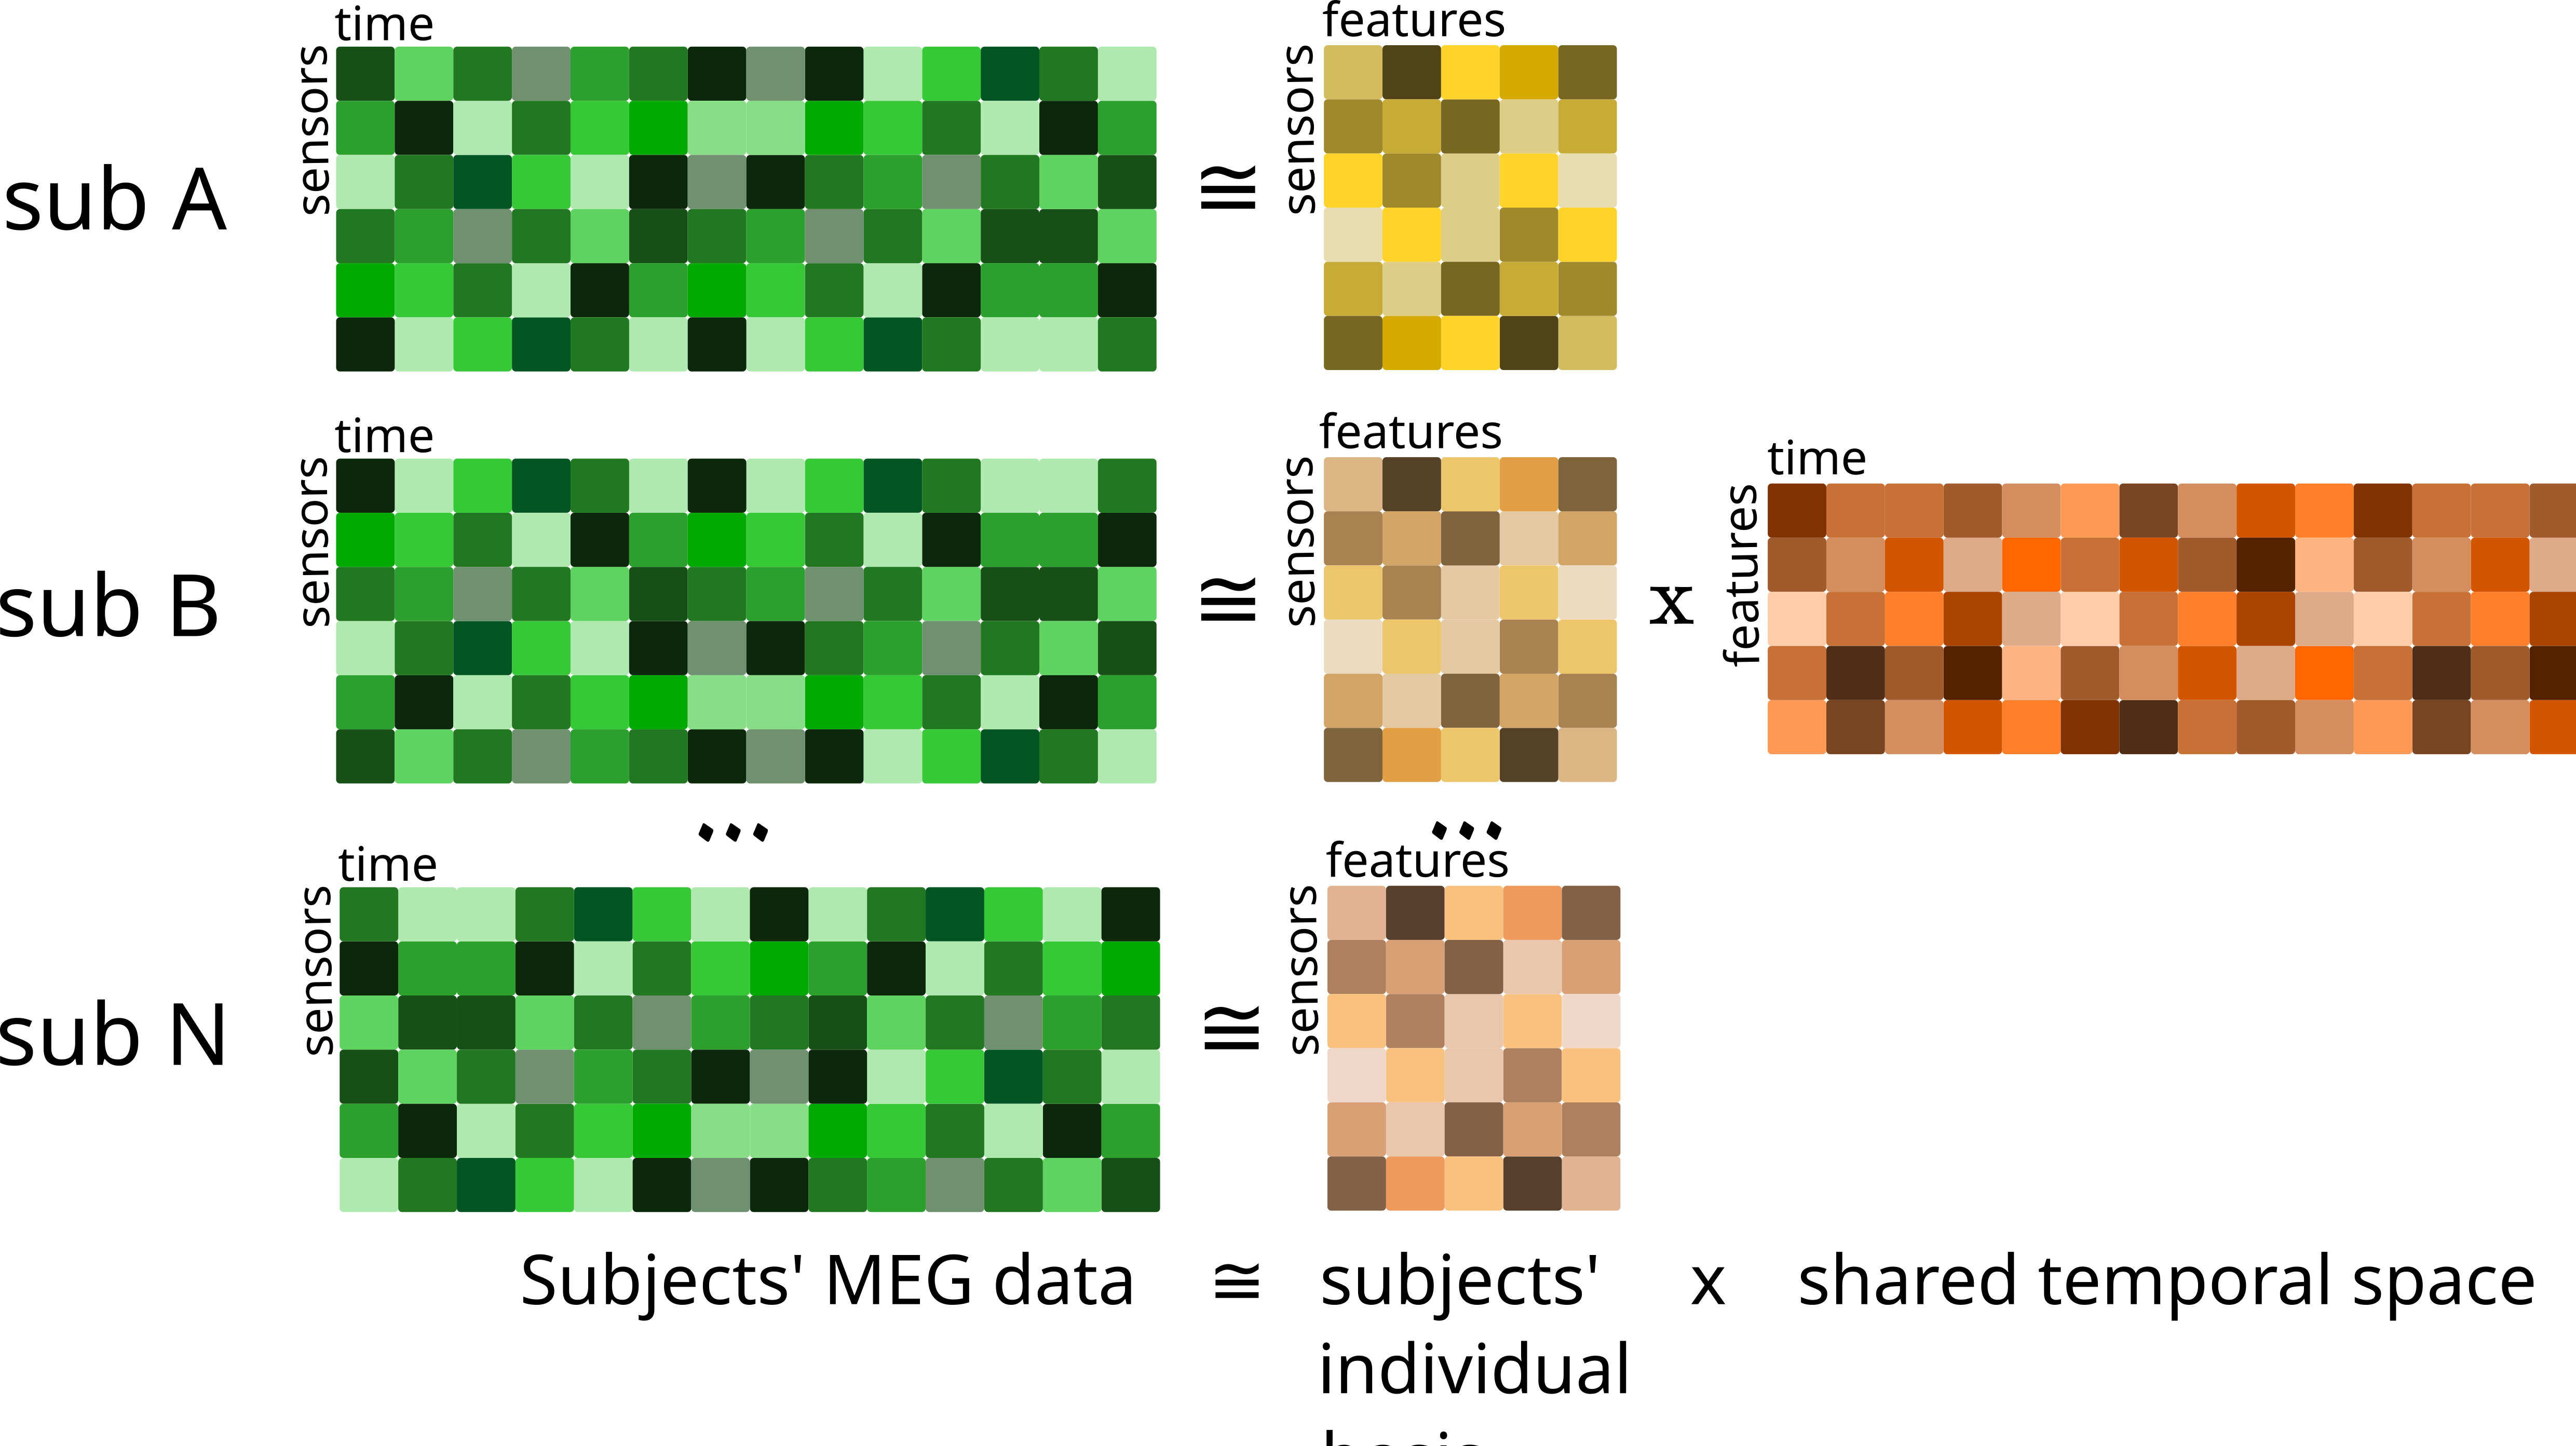
\includegraphics[width=0.9\textwidth]{memento/srm/srm_basics_3.png}
	\caption[SRM overview]{SRM overview: Sensor-by-time matrices are decomposed into a orthogonal subject specific basis matrix (sensor-by-features), a common shared feature matrix (features-by-time), and a subject-specific error}
	\label{fig:srm-basics-multi}
\end{figure}

% to do: probabilistic shared response modeling

\subsubsection{Sanity checks}

While \gls{SRM} is successfully and widely used with fMRI data (cite Elizabeth), in particular for naturalistic acquisitions with free-viewing tasks and movie stimuli (cite Sam), the method is only rarely used in \gls{meg}.
Thus the methods' utilities was first tested with a number of analyses intended to serve as sanity checks.

The first sanity check was whether basic stimulus properties are retained in the lower-dimensional data.
For this, we used the different probability and magnitude values encoded as visual properties in the stimulus.
In total, we included nine different unique combinations of probability and magnitude
% trial ordering

We normalized epoch data by z-scoring each epoch within sensors.
For this, a shared response model was trained on a subset of data.
Next, we calculated the correlation distance between the shared response during one type of trial to al other trial types, for both the left and the right stimulus option.


\section{Shared response modeling in spectral space}

MEG signal consists of oscillations with an amplitude, a frequency, and a phase.
Frequency, usually measured in hertz (Hz), is the number of times a specified event occurs within a specified time interval, while amplitude is the height, force or power of the wave, and power is the squared amplitude.
Phase involves the relationship between two or more signals that share the same frequency and describes the relationship between the position of the amplitude crests and troughs of two waveforms, measured in distance, time, or degrees.
If the peaks of two signals with the same frequency are in exact alignment at the same time, they are said to be in phase.
Conversely, if the peaks of two signals with the same frequency are not in exact alignment at the same time, they are said to be out of phase.
While shared response modeling, just like similar methods of hyper alignment [CITE], relies on the assumption that different participants display similar cognitive processes in response to the same tasks or stimuli [CITE], the exact timing or duration of such shared activity is subject to intra- and interindividual variation, and thus not necessarily phase-locked. [CITE]
[Link this to decision making tasks and previous methodological developments, such as Hidden Markov Models]

Spectral analysis consists of deconstructing a time domain signal of a given length into its constituent oscillatory components using Fourier analysis.
The resulting power spectrum displays a spectral decomposition, with the frequency domain of the oscillations on the x axis, and the amplitude on the y axis.
Thus, the signal is expressed as a function of frequency rather than time.
Such a transformation from a time-resolved representation of data to a representation in the frequency domain can be used to find shared signals with different temporal signatures [CITE probably every introductory MEG book].
Importantly, the model bases of an \gls{SRM} assign weights to sensors regardless of whether they contribute to a shared signal in time-resolved or spectral space.
Therefore, we can fit a shared response model on spectral data to find shared frequency components, but then use the model basis to transform time-resolved data (see Figure \ref{fig:spectral-srm}).
This not only allows the visualization of shared components as a time series, but also easier interpretation of components in the context of the experimental paradigm.


\begin{figure}
	\centering
	\begin{subfigure}{0.9\textwidth}
		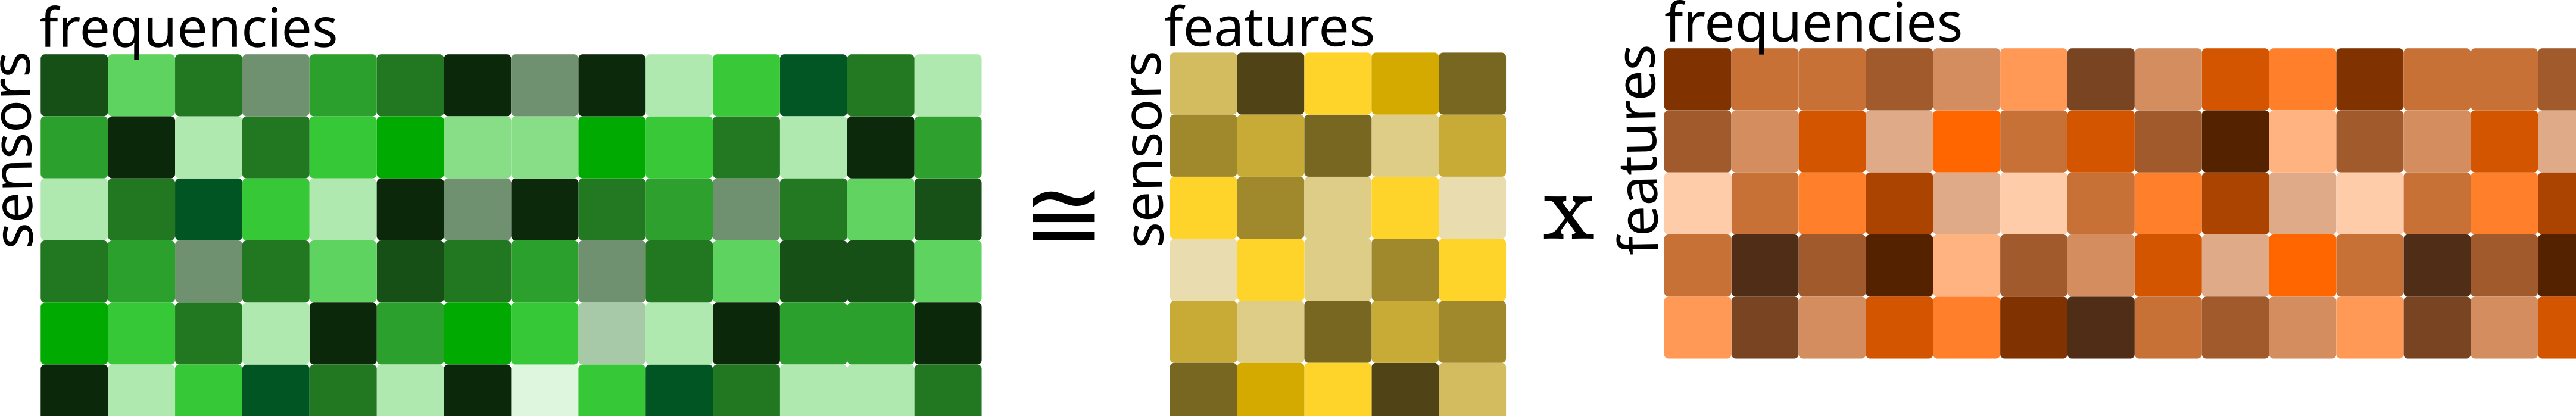
\includegraphics[width=\textwidth]{memento/spectral_srm/spectral_srm_basics_1.png}
		\caption{Fitting the shared response model on spectral data}
		\label{fig:spectral-srm1}
	\end{subfigure}
	\begin{subfigure}{0.9\textwidth}
		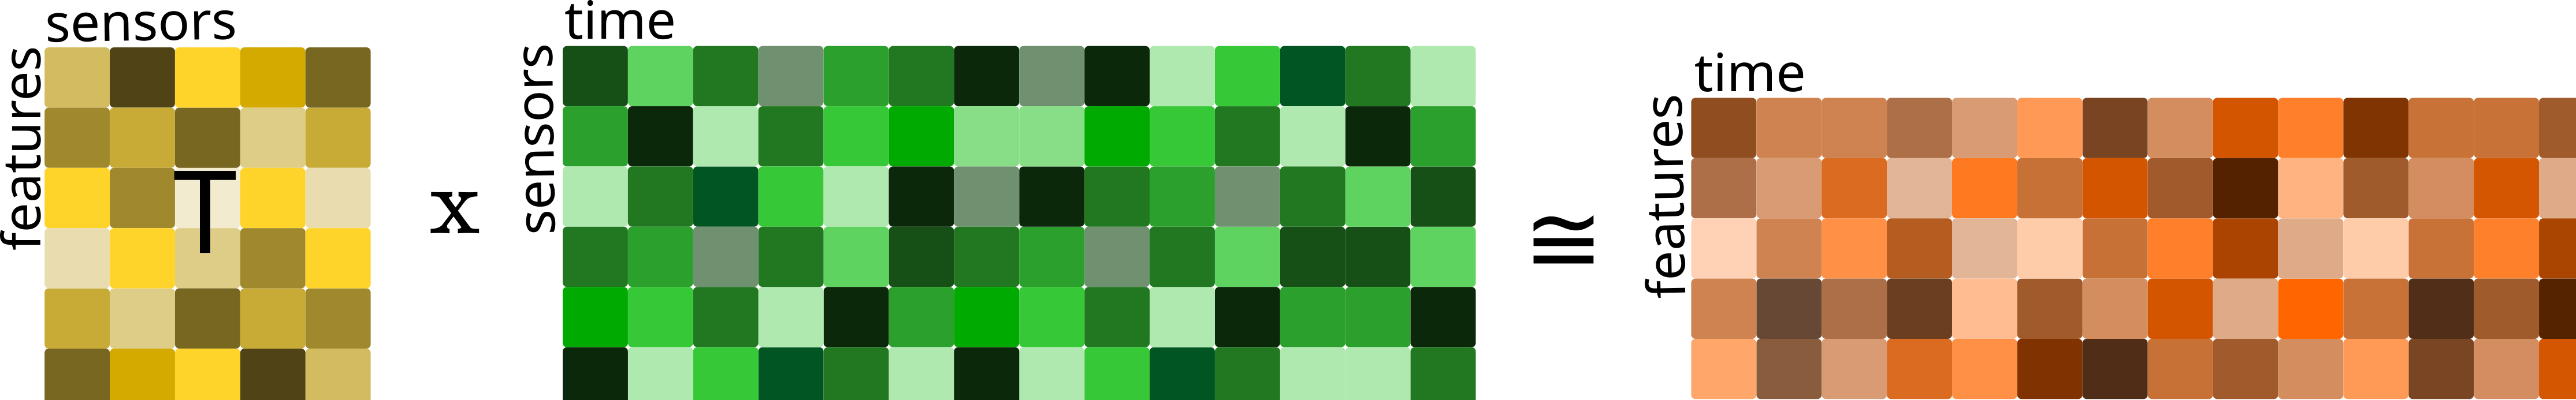
\includegraphics[width=\textwidth]{memento/spectral_srm/spectral_srm_basics_2.png}
		\caption{Transforming time resolved data into the shared space}
		\label{fig:spectral-srm2}
	\end{subfigure}
	\caption[Spectral shared response modeling]{Spectral shared response modeling: A shared response model decomposes spectral neural data (\ref{fig:spectral-srm1}, green) into a shared spectral space (features by frequencies; orange) and subject-specific basis (sensors by features; yellow). Because the subject specific bases transform sensor data independent on whether it is time resolved or spectral, they can be used to transform time resolved data (\ref{fig:spectral-srm2}; green) into time courses of the shared response spaces features.}
	\label{fig:spectral-srm}
\end{figure}

\subsection{Simulation study}


\begin{figure}
	\begin{subfigure}{1.0\textwidth}
		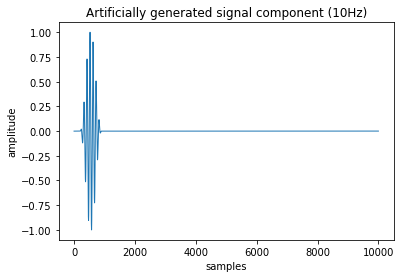
\includegraphics[width=.5\textwidth]{memento/simulation/sim_0.png}
		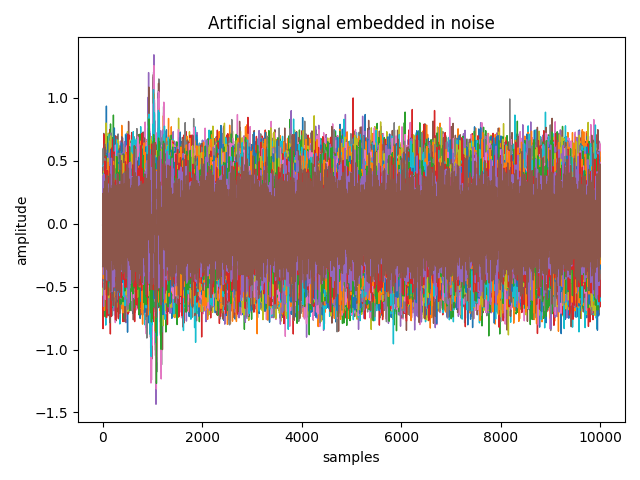
\includegraphics[width=.46\textwidth]{memento/simulation/sim_10.png}
	\end{subfigure}
	\caption{An artificial signal with 100000 samples and a 1000 sample spanning 10Hz main frequency component, pure (left) or partially embedded into 306 sensors with Gaussian noise (right). Roughly 20 percent of sensors contain the main signal in varying amounts, mirroring how brain signals are only present in certain sensors, and only in different strengths.}
	\label{fig:sim_artificial_signal}
\end{figure}

The following basic simulation illustrates the method:
In order to simulate \gls{meg} data from several subjects with a common frequency component that occurs at different points in time, we generate one ``ground truth'' signal with the same frequency and wave form, and embed it partially into 306 artificial sensors with Gaussian noise (Figure \ref{fig:sim_artificial_signal}).
To mirror how brain signals are only present in certain sensors and not with the same strength everywhere, only a fixed amount of sensors receives the signal.
For each sensor with a signal, a random weight between is drawn that determines the strength with which the signal is scaled.
This is repeated for N artificial subjects, but with a different random phase offset in the signal for each.
If the \gls{SRM} is successful, the shared response should reflect the ground truth signal despite phase offsets, and the subject-specific model bases should reflect the magnitudes of the weights for each sensor.\\
Using this data as the basis for shared response modeling, we now fit a probabilistic \gls{SRM} with $k=10$ features to recover the 10Hz signal as a shared component - either on time resolved data (Figure \ref{fig:sim-timeresolved}), or after transforming the data into its frequency spectrum (Figure \ref{fig:sim-spectral}).\\
When fit on time resolved data with phase shifts, the resulting shared space consists of components that differentially picked up signals from one or more participants, but represent it in a time series of repeated or overlapping signals.
This makes an interpretation of individual components difficult (Figure \ref{fig:sim-timeresolved-shared}).
The sensor weights that the model estimates for each component also do not show a clear association with the true weights used in the generation of the artificial data (Figure \ref{fig:sim-timeresolved-weights}).
In other words, with phase shifts between individual simulations' signals, different components of the shared space capture several participants' signals, but no \textit{general} ground truth signal.

\begin{figure}
	\begin{subfigure}{.49\textwidth}
		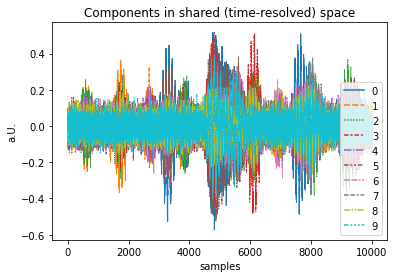
\includegraphics[width=\textwidth]{memento/simulation/sim_3.png}
		\caption{Shared space from time-resolved data}
		\label{fig:sim-timeresolved-shared}
	\end{subfigure}
	\begin{subfigure}{0.49\textwidth}
		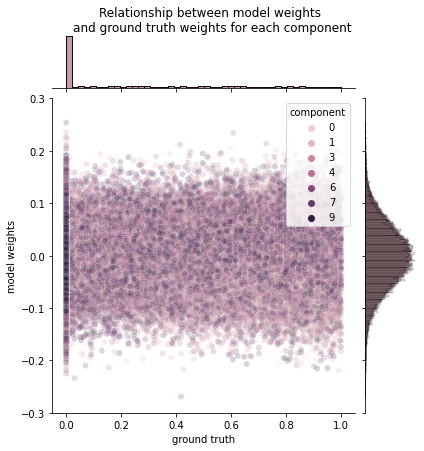
\includegraphics[width=\textwidth]{memento/simulation/sim_4.png}
		\caption{Recovered versus true weights}
		\label{fig:sim-timeresolved-weights}
	\end{subfigure}
	\caption{Outcome of fitting an \gls{SRM} on time resolved data with phase shifts: The components in shared space fail to capture a single ground truth, but show several subject's signals as consecutive or overlapping activity. The relationship between model weights and ground truth weights appears mostly random.}
	\label{fig:sim-timeresolved}
\end{figure}


However, transforming the signal into its frequency components, the spectral space, removes timing information, and with it, the phase offsets.
While the components in spectral space are not easy to interpret or differentiate (see Figure \ref{fig:sim-spectral-shared}), the scatterplot reveals that certain components' weights show a clear association to the weights used for model generation \ref{fig:sim-spectral-weights}.\\
This becomes apparent when shared components are visualized as time series by using the subject-specific weight matrices of the \gls{SRM} and individual subject's time-resolved data.
One or few components are consistently representing the original signal well across subjects, laying the basis for both identifying shared signal in phase-shifted data and interpreting the shared components resulting from it.


\begin{figure}
	\begin{subfigure}{.44\textwidth}
		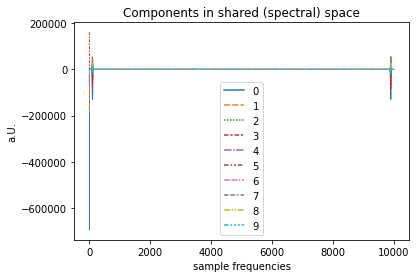
\includegraphics[width=\textwidth]{memento/simulation/sim_5.png}
			\caption{Shared space from spectral data}
		\label{fig:sim-spectral-shared}
	\end{subfigure}
	\begin{subfigure}{0.49\textwidth}
		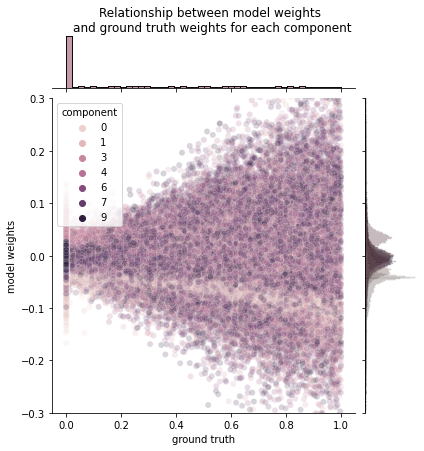
\includegraphics[width=\textwidth]{memento/simulation/sim_6.png}
			\caption{Recovered versus true weights}
		\label{fig:sim-spectral-weights}
	\end{subfigure}
	\hfill
	\begin{subfigure}{1.\textwidth}
		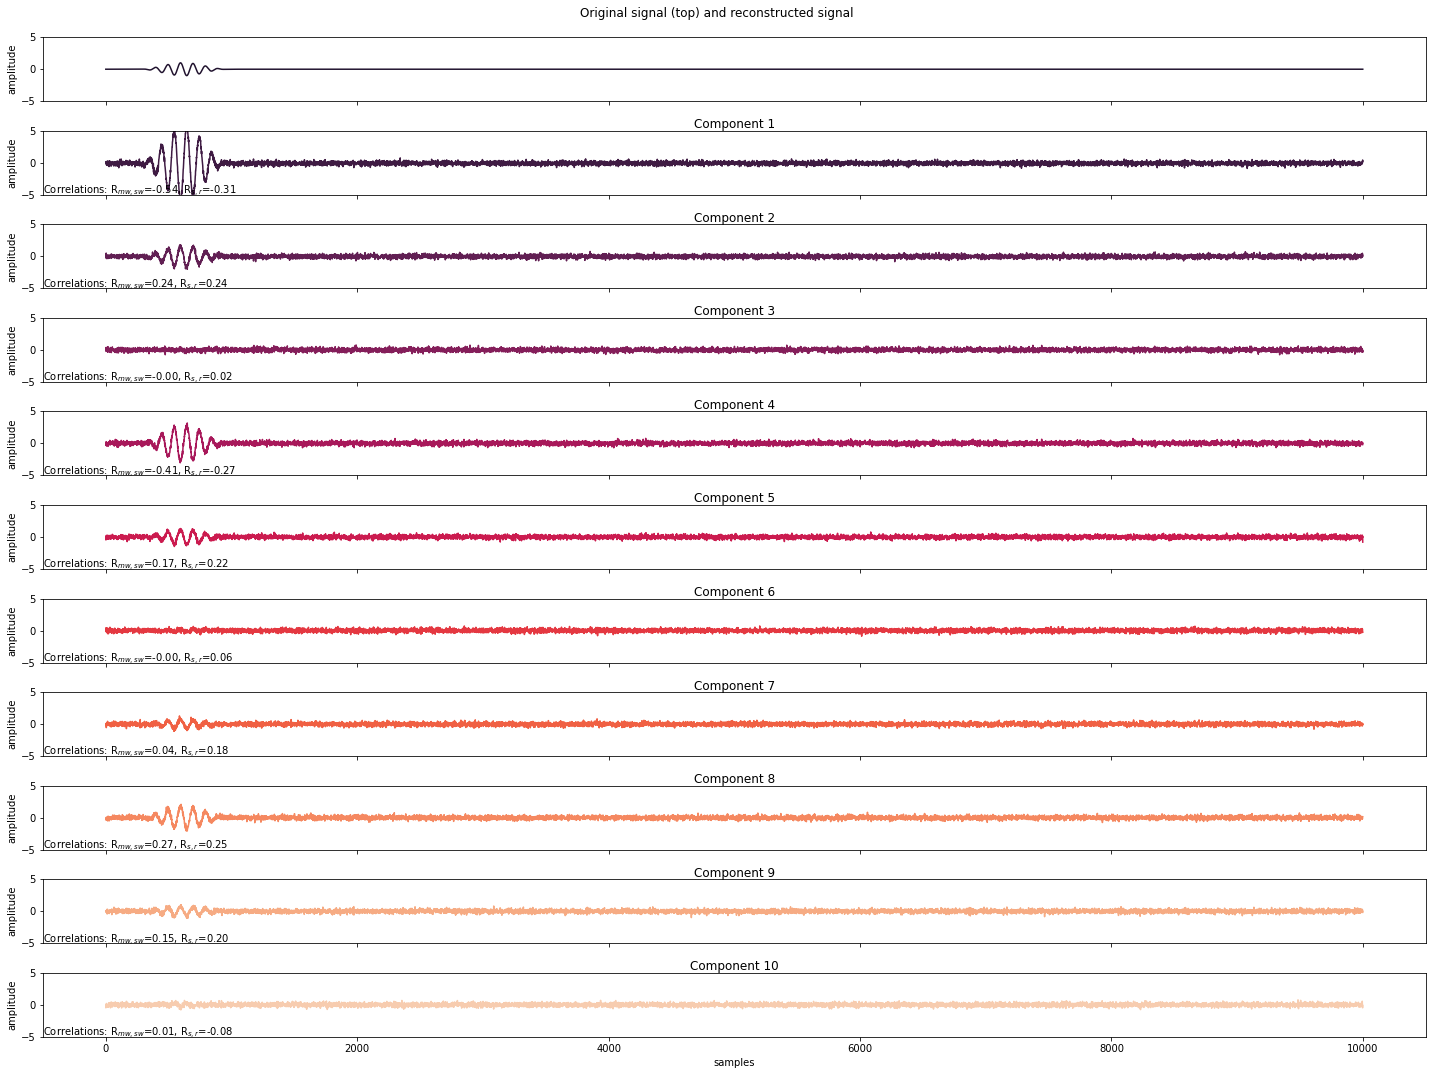
\includegraphics[width=.45\textwidth]{memento/simulation/sim_7.png}
		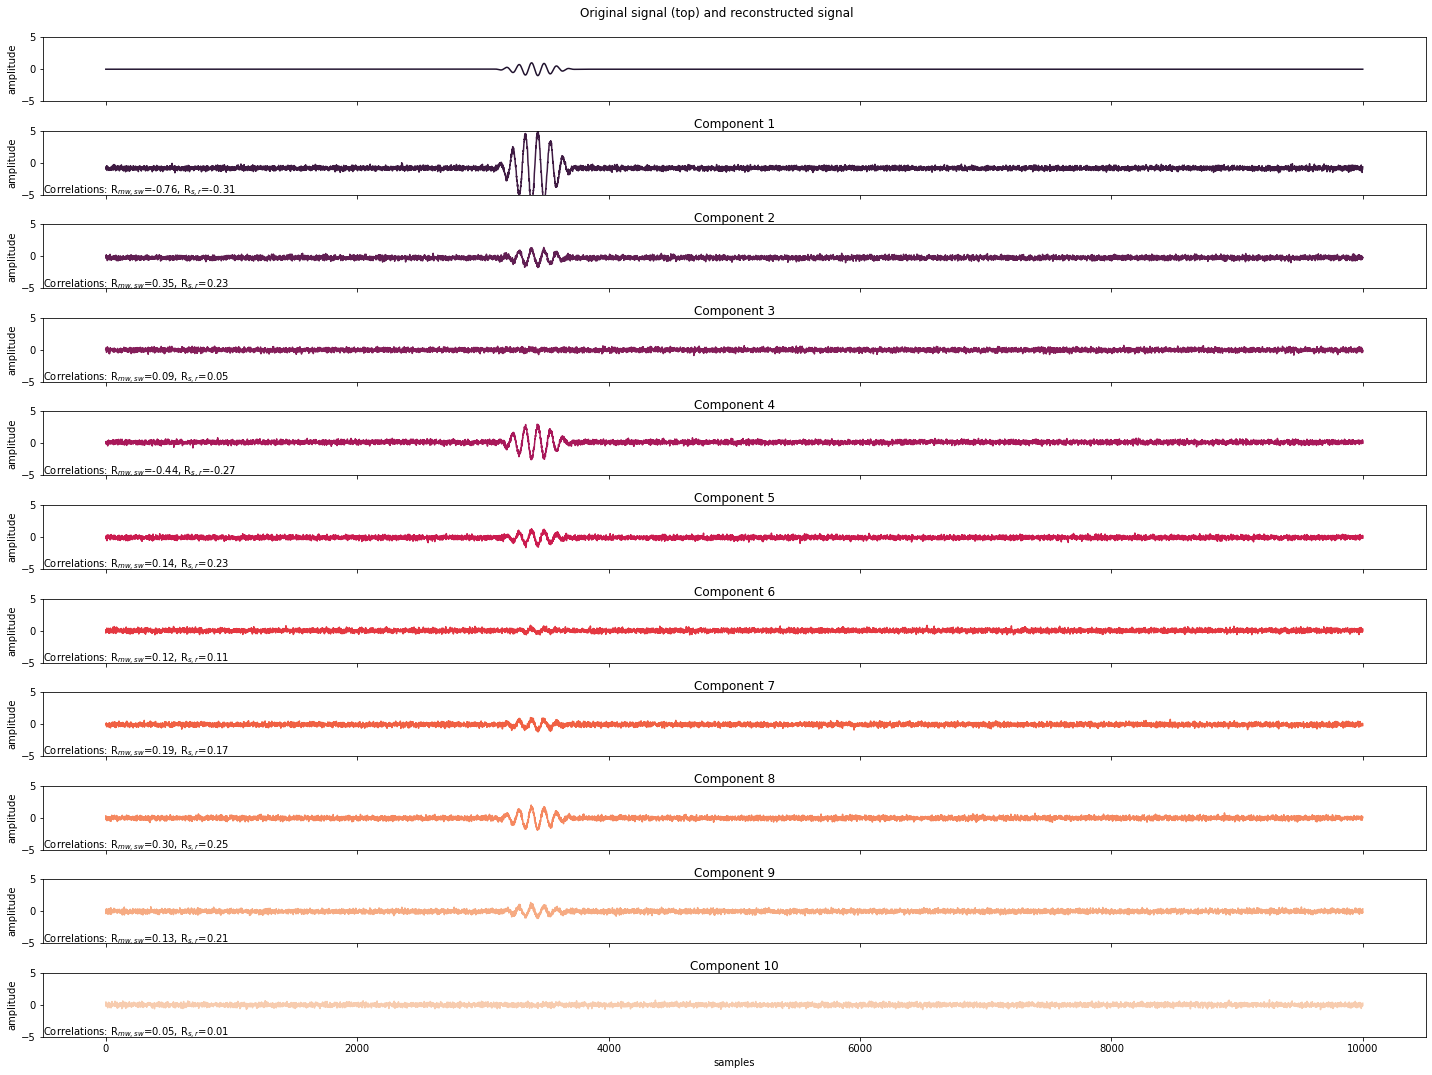
\includegraphics[width=.45\textwidth]{memento/simulation/sim_8.png}
		\caption{Shared components from \ref{fig:sim-spectral-shared}, visualized by transforming time resolved data of two different subjects}
		\label{fig:sim-spectral-transformed}
	\end{subfigure}
	\caption{Outcome of fitting an \gls{SRM} on spectrally transformed data: The components in shared space are spectral and difficult to interpret. But the relationship between model weights and ground truth weights clearly captures an association for some of the $k=10$ components. When time-resolved data from two different subjects is transformed using the subject specific bases from the \gls{SRM}, the individual subject's offset re-emerges.}
    \label{fig:sim-spectral}
\end{figure}


\subsection{Shared response modeling in spectral space on real data}

After the simulation study demonstrated principal feasibility of the method, I subsequently applied it to the neural recordings from the memento study.
The underlying aim was to investigate how decision-relevant properties are represented in working memory throughout the delay phase.
This was done with several exploratory analysis that followed the same general principle:
In a first step, data was split into a training and a test set.
For this, epochs were shuffled and randomly drawn to not introduce experiment fatigue as a confound.
A probabilistic shared response model was then fit on the spectrally transformed training data, yielding a shared spectral space (features by frequencies) and subject-specific basis (sensors by features) (\ref{fig:spectral-srm1}).
Importantly, the model had never seen the test data.
Using the subject-specific bases, the time-resolved test data was then transformed in the shared space while retaining the temporal resolution (\ref{fig:spectral-srm2}) to visualize the components the shared response model found.





\pagebreak

\section{Temporal decoding}

From Grootswagers et al. (2017): MVPA for MEG/EEG
The term “multivariate pattern analysis” (or MVPA) en-
compasses a diverse set of methods for analyzing neuro-
imaging data. The common element that unites these
approaches is that they take into account the relation-
ships between multiple variables (e.g., voxels in fMRI or
channels in MEG/EEG), instead of treating them as inde-
pendent and measuring relative activation strengths. The
term “decoding” refers to the prediction of a model from
the data (“encoding” approaches do the reverse, predict-
ing the data from the model, reviewed in Naselaris, Kay,
Nishimoto, \& Gallant, 2011; see also, e.g., Ding \& Simon,
2012, for an example of encoding models for MEG). The
most common application of decoding in cognitive neu-
roscience is the use of machine learning classifiers (e.g.,
correlation classifiers (Haxby et al., 2001) or discriminant
classifiers (Carlson et al., 2003; Cox \& Savoy, 2003) to
identify patterns in neuroimaging data, which correspond
to the experimental task or stimulus. The most popular
applications of MVPA are decoding (for recent reviews on
fMRI decoding, see e.g., Haynes, 2015; Pereira et al., 2009)
and, more recently, representational similarity analysis
(RSA: Kriegeskorte \& Kievit, 2013).

\subsection{machine learning concepts in scikit-learn}

\texttt{y} is the \textit{target}, also called \texttt{outputs}, \texttt{responses}, \texttt{label} or \texttt{ground truth}.¸ Its the \texttt{dependent variable} in supervised learning, passed to an \texttt{estimator}'s fit method as y.
\texttt{X} is the observed data. Its number of rows are the number of \texttt{samples}.
\texttt{features} are the individual elements of a vector representing a sample. In a data matrix, features are represented as columns. Elsewhere features are also known as attributes, predictors, regressors, or independent variables.
\texttt{samples} typically denote a single feature vector. Elsewhere, a sample is called an instance, data point, or observation. \texttt{n\_samples} indicates the number of samples in a dataset, being the number of rows in a data array \texttt{X}


A \texttt{classifier} is a predictor with a finite set of discrete possible output values, and must implement "fit", "predict", and "score" methods, and could implement "decision\_function", "predict\_proba" and "predict\_log\_proba" methods.
An \texttt{estimator} is an object that manages the estimation and decoding of a model. An estimators fit method takes samples X, target y, and sample properties (e.g., weights). Once fitted, the "predict\_proba" method can return probability estimates for each class from some input data X. A \texttt{score} is a method that evaluates predictions on a given dataset, returning a single

\texttt{evaluation metrics} accept a ground truth and a prediction (e.g., output of predict, predict\_proba, etc)

\texttt{Transformers} (or \texttt{transforms}) can clean, reduce, expand, or generate feature representation.
 is
\texttt{Pipelines} sequentially chain transforms with a final estimator, and reduce the possibilities of forgetting transformations that could lead to inconsistent preprocessing applications between training and testing data and of leaking test data into training data. The purpose of a pipeline is to assemble several steps that can be cross-validated together whiule

\section{Results}
\pagebreak

